\documentclass[12pt,oneside,openany,pagenumber=footcenter]{book}
%\documentclass[a4paper,10pt]{report}

\usepackage[utf8]{inputenc}
\usepackage{lmodern}
\usepackage[T1]{fontenc}
\usepackage{amsfonts}
\usepackage{amsmath}

\usepackage{fontenc}
\usepackage{graphicx}
\usepackage{graphics}
\usepackage{graphicx}
\usepackage{hyperref}
\usepackage{makeidx}

\newtheorem{definition}{Definition}[section]
\newtheorem{HLPpoznamka}{Note}[section]
\newtheorem{HLPpriklad}{Example}[section]
\newtheorem{HLPcvicenie}[HLPpriklad]{Exercise}
\newtheorem{HLPdokaz}{Proof}[section]
\newtheorem{zadanie}{Task}[section]
\newenvironment{poznamka}{\begin{HLPpoznamka}\rm}{\end{HLPpoznamka}}
\newenvironment{example}{\begin{HLPpriklad}\rm}{\end{HLPpriklad}}
\newenvironment{cvicenie}{\begin{HLPcvicenie}\rm}{\end{HLPcvicenie}}
\newenvironment{dokaz}{\begin{HLPdokaz}\rm}{\end{HLPdokaz}}
\newtheorem{veta}{Theorem}[section]
\newtheorem{lemma}[veta]{Lemma}
\newtheorem{dosledok}[veta]{Corollary}
\newtheorem{teza}[veta]{Proposition}


\pagestyle{headings}

\bibliographystyle{unsrt}

\def\indexname{Register}
% pekne pokope definujeme potrebne udaje
\def\mftitlea{Biologicky motivované výpočtové modely}
\def\mftitle{\mftitlea}
\def\mfthesistype{Dizertačná práca}
\def\mfauthor{Michal Kováč}
\def\mfadvisor{doc. RNDr. Damas Gruska, PhD.}
\def\mfplacedate{Bratislava, 2011}


\ifx\pdfoutput\undefined\relax\else\pdfinfo{ /Title (\mftitle) /Author (\mfauthor) /Creator (PDFLaTeX) } \fi

\def\eps{\varepsilon}
\def\goodgap{\hspace{\subfigcapskip}}
\makeindex

\begin{document}
\frontmatter
\thispagestyle{empty}
\begin{minipage}{0.20\textwidth}

\includegraphics[width=0.9\textwidth]{img/comenius_half.png}
\end{minipage}
\begin{minipage}{0.79\textwidth}
\begin{center}
\sc Katedra Informatiky \\
Fakulta Matematiky, Fyziky a Informatiky \\
Univerzita Komenského, Bratislava
\end{center}
\end{minipage}

\vfill
\begin{center}
\begin{minipage}{0.8\textwidth}
\hrule
\bigskip\bigskip
\centerline{\LARGE\sc\mftitlea}
\smallskip
\centerline{(\mfthesistype)}
\bigskip
\bigskip
\centerline{\large\sc\mfauthor}
\bigskip\bigskip
\hrule
\end{minipage}
\end{center}
\vfill
{\bf Vedúci:} \mfadvisor
\hfill\mfplacedate
\eject
\eject

\thispagestyle{empty}
{~}\vspace{12cm}

{~}\vspace{12cm}

\begin{minipage}{0.25\textwidth}~\end{minipage}
\begin{minipage}{0.69\textwidth}
I hereby declare that this submission is my own work and that, to the best of my knowledge and belief, it contains no material previously published or written by another person nor material which to a substantial extent has been accepted for the award of any other degree or diploma of the university or other institute of higher learning, except where due acknowledgment has been made in the text.

\bigskip\bigskip

\hfill\hbox to 6cm{\dotfill}
\end{minipage}

\chapter*{Acknowledgements}

I am very grateful to all the people I had the privilege to work with, especially I would like to thank my advisor RNDr. Damas Gruska PhD. for his constant interest, encouragement and help that I deeply appreciate.
The present work was possible due to many beneficial consultations and intensive cooperation.

I would also like to thank to the members of Laboratory of Comparative and Functional Genomics of Eukaryotic Organelles and their head, Prof. Ľubomír Tomáška for familiarization with the work of biologists.

I thank to my family, colleagues, teammates and all the friends who supported me especially last weeks before the deadlines for their patience, support and understanding\footnote{Understanding that they will propably never understand my work;)}

% Osobitná vďaka patrí vedúcemu diplomovej práce doc. RNDr. Damasovi Gruskovi PhD. za cenné rady, námety, podnetné pripomienky a všestrannú pomoc, ktorú si hlboko vážim. Len vďaka mnohým prínosným konzultáciam a intenzívnej spolupráci som bol schopný napísať toto dielo. Nesmiem zabudnúť ani na RNDr. Branislava Rovana, CSc. a spolužiakov za to, že si na dizertačnom seminári našli čas, aby si vypočuli moju prezentáciu dizertačnej práce. Ďalšie poďakovania venujem rodičom a známym, ktorí to so mnou dokázali vydržať posledné týždne pred odovzdaním.

% !TEX root = diz.tex
\chapter*{Abstract}
\begin{description} \itemsep1pt \parskip0pt \parsep0pt
  \item[Author:] \mfauthor
  \item[Title:] \mftitle
  \item[University:] Comenius University in Bratislava
  \item[Faculty:] Faculty of Mathematics, Physics and Informatics
  \item[Department:] Department of Applied Informatics
  \item[Supervisor:] \mfadvisor
\end{description}

This work discusses the research in the membrane systems, an emerging field of natural computing. Many variants of membranes systems have already been studied, most of them uses parallel rewriting and are computationally complete. Various sequential models have been proposed, however, in many cases they are weaker than their parallel variant.

We propose some other sequential models, provide universality proofs for them and suggest further research.

\begin{description}
  \item[Keywords:] Computation models inspired by biology, Membrane systems, P systems
\end{description}

\chapter*{Abstrakt}
\begin{description} \itemsep1pt \parskip0pt \parsep0pt
  \item[Autor:] \mfauthor
  \item[Názov dizertačnej práce:] \mftitle
  \item[Škola:] Univerzita Komenského v Bratislave
  \item[Fakulta:] Fakulta matematiky, fyziky a informatiky
  \item[Katedra:] Katedra aplikovanej informatiky
  \item[Vedúci dizertačnej práce:] \mfadvisor
  \item \mfplacedate
\end{description}

V tejto práci sa zaoberáme výskumom v oblasti membránových systémov. Veľa variantov už bolo preskúmaných, väčšinou pri výpočte používajú paralelizmus a sú Turingovsky úplné. Navrhlo sa aj veľa sekvenčných modelov, ale väčšina z nich má slabšiu výpočtovú silu ako ich paralelný variant.

V druhej časti predkladáme niektoré sekvenčné modely, u ktorých dokazujeme Turingovu úplnosť a navrhujeme modely, ktoré plánujeme preskúmať v rámci dizertačnej práce.

\begin{description}
  \item[Kľúčové slová:] Výpočtové modely inšpirované biológiou, Membránové systémy, P systémy
\end{description}
\tableofcontents{}
\listoffigures{}
\listoftables{}

\mainmatter

\chapter*{Introduction} % (fold)
\label{cha:introduction}
% !TEX root = diz.tex
\addcontentsline{toc}{chapter}{Introduction}

There are a lot of areas in the theoretical computer science that are motivated by other science fields. Computation models motivated by biology forms a large group of them. They include neural networks, computational models based on DNA evolutionary algorithms, which have already found their use in computer science and proved that it is worth to be inspired by biology. L-systems are specialized for describing the growth of plants, but they have also found the applications in computer graphics, especially in fractal geometry. Other emerging areas are still awaiting for their more significant uses.

One of them is the membrane computing \cite{Paun10OxfordHandbookMembraneComputing}. It is relatively young field of natural computing - in comparison: neural networks have been researched since 1943 and membrane systems since 1998 \cite{Paun98}.

Membrane systems (P systems) are distributed parallel computing devices inspired by the structure and functionality of cells. Recently, many P system variants have been developed in order to simulate the cells more realistically or just to improve the computational power.

We will start by an introduction of some natural computing areas including models inspired by biology in Chapter \ref{cha:natural_computing}. In Chapter \ref{cha:preliminaries} we recall some computer science basic notions that we will use through the work. P systems are formally presented in Chapter \ref{cha:p_systems}, with the current state of the research in their variants, overview of software simulator MeCoSym and various case studies.

In Chapter \ref{cha:on_the_edge_of_universality_of_sequential_p_systems} we will present the current state of our work, mainly from theoretic viewpoint (computational power, decidability of behavioral properties), including the published results in sections \ref{sec:inhibitors}, \ref{sec:active_membranes} and \ref{sec:notions_from_reaction_systems}.


% chapter introduction (end)

\part{Overview of the current state of research} % (fold)
\label{part:overview_of_the_current_state_of_research}


\chapter{Preliminaries} % (fold)
\label{cha:preliminaries}
This chapter is about some basic notions of computer science which will be used through the work. We start by defining formal languages and basic models (grammars, machines) that define language families and end by defining multiset languages.

\section{Formal languages} % (fold)
\label{sec:formal_languages}

Our study is based on the classical theory of formal languages. We will recall some definitions:

\begin{definition}
An {\bf alphabet} is a finite nonempty set of symbols.
\end{definition}

\begin{definition}
A {\bf string} over an alphabet is a finite sequence of symbols from alphabet.
\end{definition}

The length of the string $s$ is denoted by $|s|$. We denote by $V^*$ the set of all strings over an alphabet $V$. By $V^+$ = $V^* - \{\eps\}$ we denote the set of all nonempty strings over V.

\begin{definition}
A {\bf language} over the alphabet $V$ is any subset of $V^*$.
\end{definition}

\begin{definition}
A {\bf family of languages} is a set of languages.
\end{definition}


\section{Formal grammars} % (fold)
\label{sec:formal_grammars}

\begin{definition}
A {\bf formal grammar} is a tuple $G = (N,T,P,\sigma)$, where
\begin{itemize}
  \item $N, T$ are disjoint alphabets of non-terminal and terminal symbols,
  \item $\sigma\in N$ is the initial non-terminal,
  \item $P$ is a finite set of rewriting rules of the form $u\rightarrow v$, with $u\in (N\cup T)^*N(N\cup T)^*$ and $v\in (N\cup T)^*$.
\end{itemize}
\end{definition}

\begin{definition}
A {\bf rewriting step} in the grammar $G$ is a binary relation $\Rightarrow$ on $(N\cup T)^*$, where $x\Rightarrow y$ only if $\exists w_1, w_2\in (N\cup T)^+$ and a rule $u\rightarrow v \in P$ such that $x=w_1uw_2$ and $y=w_1vw_2$.
\end{definition}

\begin{definition}
Language defined by a grammar $G$ is a set $L(G)=\{w\in T^*|\sigma\Rightarrow w\}$.
\end{definition}

Languages that can be generated by a formal grammar are the recursively enumerable languages $RE$.

% section formal_languages (end)

% section formal_grammars (end)

\section{Chomsky hierarchy} % (fold)
\label{sec:chomsky_hierarchy}

In this section we introduce several well-known families of languages.

\begin{definition}
A {\bf regular grammar} is a formal grammar, where the rewriting rules are of the form $u\rightarrow v$, where $u\in N$ and $v\in T^*(N\cup \{\eps\})$.
\end{definition}

\begin{definition}
A {\bf regular language} is a language generated by a regular grammar. The family of regular languages is denoted $R$.
\end{definition}

\begin{definition}
A {\bf context-free grammar} is a formal grammar, where rewriting rules are of the form $u\rightarrow v$, where $u\in N$ and $v\in (N\cup T)^*$.
\end{definition}

\begin{definition}
A {\bf context-free language} is a language generated by a context-free grammar. The family of context-free languages is denoted $CF$.
\end{definition}

\begin{definition}
A {\bf context-sensitive grammar} is a formal grammar, where rewriting rules are of the form $u\rightarrow v$, where $u\in (N\cup T)^*N(N\cup T)^*$, $v\in (N\cup T)^*$ and $|u| < |v|$.
\end{definition}

\begin{definition}
A {\bf context-sensitive language} is a language generated by a context-sensitive grammar. The family of context-sensitive languages is denoted $CS$.
\end{definition}

These families of languages forms the Chomsky hierarchy by means of inclusions: $R \subset CF \subset CS \subset RE$.

% section chomsky_hierarchy (end)

\section{Matrix grammars} % (fold)
\label{sec:matrix_grammars}

\begin{definition}
A {\bf matrix grammar} is a tuple $G = (N,T,M,\sigma)$, where:
\begin{itemize}
  \item $N, T$ are disjoint alphabets of non-terminal and terminal symbols,
  \item $\sigma\in N$ is the initial non-terminal,
  \item $M$ is a finite set of matrices, which are sequences of context-free rules of the form $u\rightarrow v$, where $u\in N$ and $v\in (N\cup T)^*$.
\end{itemize}
\end{definition}

\begin{definition}
A {\bf rewriting step} $x\Rightarrow y$ holds only if there is a matrix $(u_1\rightarrow v_1, u_2\rightarrow v_2, \ldots, u_n\rightarrow v_n) \in M$ such that for each $1\leq i\leq n$ the following holds: $x_i = x_i^{\prime}u_ix_i^{\prime\prime}$ and $x_{i+1} = x_i^{\prime}v_ix_i^{\prime\prime}$, where $x_i, x_i^{\prime}, x_i^{\prime\prime} \in (N\cup T)^*$ and $x_1 = x$ and $x_{n+1} = y$.
\end{definition}

\begin{example}
Consider the matrix grammar $G=(\{\sigma, X,Y\}, \{ a,b,c\}, M, \sigma)$, where $M$ contains three matrices: $[S\rightarrow XY], [X\rightarrow aXb, Y\rightarrow cY], [X\rightarrow ab, Y\rightarrow c]$. There are only context-free rules, yet the grammar generate the context-sensitive language $\{a^nb^nc^n|n\geq 1\}$.
\end{example}

The family of matrix grammars is denoted $MAT$.

It is known that $CF \subset MAT \subset RE$. Interestingly, $MAT \cap {a}^* \subset R$ (see \cite{Besozzi:PhD:2004}).

% section matrix_grammars (end)

\section{Register machines} % (fold)
\label{sec:register_machines}

% We will use the notion of register machine as defined in our article

\begin{definition}
  A {\bf $n$-register machine} is a tuple $M = (n,P,i,h)$, where:
  \begin{itemize}
    \item $n$ is the number of registers,
    \item $P$ is a set of labeled instructions of the form $j : (op(r),k,l)$, where $op(r)$ is an operation on register $r$ of $M$, and $j$, $k$, $l$ are labels from the set $Lab(M)$ (which numbers the instructions in a one-to-one manner),
    \item $i$ is the initial label, and
    \item $h$ is the final label.
  \end{itemize}
\end{definition}

The machine is capable of the following instructions:
\begin{itemize}
\item $(add(r),k,l)$ : Add one to the contents of register $r$ and proceed to instruction $k$ or to instruction $l$; in the deterministic variants usually considered in the literature we demand $k = l$.
\item $(sub(r),k,l)$ : If register $r$ is not empty, then subtract one from its contents and go to instruction $k$, otherwise proceed to instruction $l$.
\item $halt$ : This instruction stops the machine. This additional instruction can only be assigned to the final label $h$.
\end{itemize}

A deterministic $m$-register machine can analyze an input $(n_1,\dots,n_m)\in N_0^m$ in registers 1 to $m$, which is recognized if the register machine finally stops by the halt instruction with all its registers being empty (this last requirement is not necessary). If the machine does not halt, the analysis was not successful.

% section register_machines (end)

\section{Lindenmayer systems} % (fold)
\label{sec:lindenmayer_systems}

In 1968, a Hungarian botanist and theoretical biologist Aristid Lindenmayer introduced \cite{Lindenmayer68} a new string rewriting algorithm named Lindenmayer systems (or L-systems for short). They are used by biologists and theoretical computer scientists to mathematically model growth processes of living organisms, especially plants. The difference with Chomsky grammars is that rewriting is parallel, not sequential.

The simplest version of L-systems assumes that the development of a cell is free of influence of other cells.
This type of L-systems is called $0L$ systems, where ``0'' stands for zero-sided communication between cells.

\begin{definition}
A $0L$ system is a triple $(\Sigma, P, \omega)$, where $\Sigma$ is an alphabet, $\omega$ is a word over $\Sigma$ and $P$ is a finite set of rewriting rules of the form $a\rightarrow x$, where $a\in\Sigma, x\in\Sigma^*$.
\end{definition}

It is assumed there is at least one rewriting rule for each letter of $\Sigma$. $0L$ system works in parallel way, so all the symbols are rewritten in each step.

\begin{example}
Consider a $0L$ system with alphabet $\Sigma = \{a,b\}$, initial word $\omega = a$ and rewriting rules $P = \{a\rightarrow b, b\rightarrow ab\}$.
Since in this system there is exactly one rule for every letter of the alphabet, the rewriting is thus deterministic and the generated words will be $\{a, b, ab, bab, abbab, \ldots \}$. 
\end{example}

$1L$ systems allows the rewriting rules to include context of size 1, so it allows for rules of type $yaz\rightarrow x$.

L-systems with tables ($T$) have several sets of rewriting rules instead of just one set. At one step of the rewriting process, rules belonging to the same set have to be applied. The biological motivation for introducing tables is that one may want different rules to take care of different environmental conditions (heat, light, etc.) or of different stages of development.

\begin{definition}
An extended ($E0L$) system is a pair $G_1 = (G, \Sigma_T)$, where $G = (\Sigma, P, \omega)$ is an $0L$ system, where $\Sigma_T \subseteq \Sigma$, referred to as the terminal alphabet. The language generated by $G_1$ is defined by $L(G_1) = L(G)\cap \Sigma_T^*$.
\end{definition}

Such languages are called $E0L$ languages. $E0L$ languages with tables are called $ET0L$ languages.

It is known that $CF \subset E0L \subset ET0L \subset CS$ (see section \ref{sec:chomsky_hierarchy} for definitions of $CF$ and $CS$).
% section lindenmayer_systems (end)

\section{Multisets} % (fold)
\label{sec:multisets}

\begin{definition}
A multiset over a set $X$ is a mapping $M: X\rightarrow \mathbb N$.
\end{definition}

We denote by $M(x), x\in X$ the multiplicity of $x$ in the multiset $M$.

\begin{definition}
The {\bf support} of a multiset $M$ is the set $supp(M)=\{x\in X|M(x)\geq 1\}$.
\end{definition}

It is the set of items with at least one occurrence.

\begin{definition}
A multiset is {\bf empty} when its support is empty.
\end{definition}

A multiset $M$ with finite support $X = \{x_1, x_2, \ldots, x_n\}$ can be represented by the string $x_1^{M(x_1)}x_2^{M(x_2)}\ldots x_n^{M(x_n)}$.
As elements of a multiset can also be strings, we separate them with the pipe symbol, e.g. $$element|element|other\_element$$.

\begin{definition}
Multiset inclusion. We say that multiset $M_1$ is included in multiset $M_2$ if $\forall x \in X: M_1(x)\leq M_2(x)$. We denote it by $M_1\subseteq M_2$.
\end{definition}

\begin{definition}
The {\bf union} of two multisets $M_1\cup M_2$ is a multiset where $\forall x \in X: (M_1\cup M_2)(x)=M_1(x)+M_2(x)$.
\end{definition}

\begin{definition}
The {\bf difference} of two multisets $M_1-M_2$ is a multiset where $\forall x \in X: (M_1-M_2)(x)=M_1(x)-M_2(x)$.
\end{definition}

\begin{definition}
Product of multiset $M$ with natural number $n\in \mathbb N$ is a multiset where $\forall x \in X: (n\cdot M)(x)=n\cdot M(x)$.  
\end{definition}

% section multisets (end)

\section{Semilinear sets} % (fold)
\label{sec:semilinear_sets}

\begin{definition}
  A {\bf linear set} $L(c,p_1,\ldots,p_r)$ is a subset $\{c+\sum\limits_{i=1}^r|k_i\in\mathbb N\}$ of $\mathbb N^n$, where $c,p_1,\ldots,p_r\in \mathbb N^n$.
\end{definition}

We call $c$ the constant and $p_1,\ldots,p_r$ the periods of the linear set.

\begin{example}
  For $n=1$ the linear set is a subset of $\mathbb N$. For $n=1$ and $r=1$ we get an arithmetic progression.
\end{example}

\begin{example}
  $L((0,0),(0,1),(1,0))$ contains all pairs with one zero element and one non-negative element: $$\{(0,0), (1,0), (2,0), \ldots, (x,0), \ldots, (0,1), (0,2), \ldots, (0,y), \ldots\}$$.
\end{example}

\begin{definition}
  A subset of $\mathbb N^n$ is called {\bf semilinear} if it is a finite union of linear sets.
\end{definition}

\subsection{Parikh's mapping} % (fold)
\label{sec:parikh_s_mapping}

In this subsection we show how semilinear sets and multisets relate to the formal language theory. We will start with several basic definitions.

The number of occurrences of a given symbol $a\in \Sigma$ in the string $w\in \Sigma^*$ is denoted by $|w|_a$.

\begin{definition}
$\Psi_\Sigma(w)=(|w|_{a_1},|w|_{a_2},\ldots,|w|_{a_n})$ is called a {\bf Parikh image of the string} $w\in \Sigma^*$, where $\Sigma=\{a_1,a_2,\ldots a_n\}$.
\end{definition}

When referring to the Parikh mapping for a language, this should be taken to mean the mapping applied to all the words on the language. This idea is expressed in the next definition. 

\begin{definition}
For a language $L\subseteq \Sigma^*$, $\Psi_\Sigma(L)=\{\Psi_\Sigma(w)|w\in L\}$ is the {\bf Parikh image of the language} $L$.
\end{definition}

\begin{definition}
If $FL$ is a family of languages, by $PsFL$ we denote the family of Parikh images of languages in $FL$, e.g. $PsCF, PsRE$.
\end{definition}

\begin{example}
Consider an alphabet $V=\{a,b\}$ and a language $L=\{a, ab, ba\}$.
$\Psi_\Sigma(L)=\{(1,0), (1,1)\}$. Notice that Parikh image of $L$ has only 2 element while $L$ has 3 elements.
\end{example}

\begin{example}
  Consider the context-free grammar $G = (N,T,P,\sigma)$, where $N=\{A,B\}$, $T=\{a,b\}$ and with rules $P=\{\sigma\rightarrow A\sigma B|B\sigma A|ab, A\rightarrow a, B\rightarrow b\}$.

  This means that the language generated by $G$ contains strings where $a$s and $b$s can occur intermixed. But, as is clear from the language definition, the same number of $a$s and $b$s will always be present. Moreover, there will always be at least one of each letters.

  Consider the words $w_1 = aaaabbbb \in L(G)$ and $w_2 = babababa \in L(G)$. Both of these words have the same Parikh image: $\Psi_\Sigma(w_i) = (4,4)$. It is interesting to note that most information embedded in a word generated with a context-free grammar is thrown away by the Parikh mapping.
\end{example}

This loss of information is expressed in the Parikh's theorem \cite{Parikh66}, stating that the Parikh image of a context-free language is semilinear. The biggest implication of the theorem though, is that it shows that if the order of the symbols is ignored, then it is impossible to distinguish between a regular set and a context-free language \cite{Kozen97Automata}.

Another interesting result appeared in \cite{Ito69Semilinear} that every semilinear set is a finite union of disjoint linear sets.

% subsection parikh_s_mapping (end)

% section semilinear_sets (end)

\section{Petri nets} % (fold)
\label{sec:petri_nets}

Petri nets \cite{Petri62,Yen06PetriNets} were introduced by Carl Adam Petri in 1962 in his PhD thesis. A Petri net is a graphical and mathematical tool for the modeling of concurrent processes and analysis of system behavior. A Petri net is usually drawn as a directed bipartite graph with two kind of nodes. Places are represented by circles within which each small black dot denotes a token. Transitions are represented by bars. Each edge is either from a place to a transition or vice versa.

\begin{definition}
  A {\bf Petri net} is a tuple $(P, T, \varphi)$, where:
  \begin{itemize}
    \item $P$ is a finite set of places,
    \item $T$ is a finite set of transitions,
    \item $\varphi: (P\times T)\cup(T\times P)\rightarrow \mathbb N$ is a flow function.
  \end{itemize}
\end{definition}

The edges of the bipartite graph are annotated by either $\varphi(p,t)$ or $\varphi(t,p)$, where $p\in P$ and $t\in T$ are two endpoints of the arc. If $\varphi(p,t)=1$ or $\varphi(t,p)=1$, we usually omit the label.

\begin{definition}
  A {\bf marking} is a mapping $\mu: P\rightarrow \mathbb N$.
\end{definition}

The mapping $\mu$ assigns certain number of tokens to each place of the net.

\begin{definition}
  A marking $\mu_1$ {\bf covers} marking $\mu_2$, when $\forall p\in P: \mu_1(p)\geq\mu_2(p)$ - in each place there is no less tokens in $\mu_1$ than in $\mu_2$. We denote it by $\mu_1\geq\mu_2$.
\end{definition} 

\begin{definition}
  A transition $t\in T$ is {\bf enabled} at a marking $\mu$ iff $\forall p\in P, \varphi(p,t)\leq\mu(p)$.
\end{definition}

If a transition $t$ is enabled, it may fire by removing $\varphi(p,t)$ tokens from each input place $p$ and putting $\varphi(t,p^\prime)$ tokens in each output place $p^\prime$. We then write $\mu\xrightarrow{t} \mu^\prime$, where $\forall p\in P: \mu^\prime(p) = \mu(p)-\varphi(p,t)+\varphi(t,p)$.

\begin{example}
  In the Figure \ref{fig:example petri net} the Petri net has four places and two transitions. At the current marking the transition $t_1$ is enabled and the transition $t_2$ is not enabled. Firing the transition $t_1$ takes one token from the place $p_1$ and produces one token to places $p_2, p_3$ and $p_4$. In the resulting marking both transitions $t_1$ and $t_2$ are enabled.
\end{example}

\begin{definition}
  A {\bf marked Petri net} is a tuple $(P,T,\varphi,\mu_0)$, where $(P,T,\varphi)$ is a Petri net and $\mu_0$ is called the initial marking.
\end{definition}

\begin{definition}
  A sequence of transitions $\sigma = t_1\ldots t_n$ is a {\bf firing sequence} from $\mu_0$ iff $\mu_0\xrightarrow{t_1}\mu_1\xrightarrow{t_2}\ldots\xrightarrow{t_n}\mu_n$ for some markings $\mu_1,\ldots,\mu_n$. We also write $\mu_0\xrightarrow{\sigma}\mu_n$.
\end{definition}

We write $\mu_0\xrightarrow{\sigma}$ to denote that $\sigma$ is enabled and can be fired from $\mu_0$, i.e., $\mu_0\xrightarrow{\sigma}$ iff there exists a marking $\mu$ such that $\mu_0\xrightarrow{\sigma}\mu$.
The notation $\mu_0\xrightarrow{*}\mu$ is used to denote the existence of a firing sequence $\sigma$ such that $\mu_0\xrightarrow{\sigma}\mu$.

\begin{definition}
  A marking $\mu$ is reachable for a marked Petri net $\mathcal P = (P,T,\varphi,\mu_0)$ iff $\mu_0\xrightarrow{*}\mu$.
\end{definition}

\begin{definition}
  Let $\mathcal P = (P,T,\varphi,\mu_0)$ be a marked Petri net. The {\bf reachability set} of $\mathcal P$ is $R(\mathcal(P)) = \{\mu|\mu_0\xrightarrow{*}\mu\}$.
\end{definition}

A notion of reachability graph is helpful for analyzing the behavior of a Petri net as a tool for visualisation of the structure of the reachability set.

\begin{definition}
  Let $\mathcal P = (P,T,\varphi,\mu_0)$ be a marked Petri net. The {\bf reachability graph} of $\mathcal P$ is a labelled graph whose nodes are the reachable markings and edge from $\mu_1$ to $\mu_2$ is labeled with a transition $t\in T$ iff $\mu_1\xrightarrow{t}\mu_2$.
\end{definition}

\begin{figure}
  \centering
  \begin{minipage}{.4\textwidth}
    \begin{tikzpicture}
      \tikzstyle{transition}=[rectangle,thick,fill=black,minimum height=8mm]
      \node [place,tokens=3,label=above:$p_1$] (p1) {};
      \node [transition,label=above:$t_1$] (t1) [right of=p1] {}
        edge [pre] (p1);
      \node [place,tokens=0,label=right:$p_3$] (p3) [right of=t1] {}
        edge [pre] (t1);
      \node [place,tokens=0,label=right:$p_2$] (p2) [above of=p3] {}
        edge [pre] (t1);
      \node [place,tokens=0,label=right:$p_4$] (p4) [below of=p3] {}
        edge [pre] (t1);
      \node [transition,label=below:$t_2$] (t2) [below of=t1] {}
        edge [pre] (p4)
        edge [post] (p1);
    \end{tikzpicture}
    \captionof{figure}{An example Petri net}
    \label{fig:example petri net}
  \end{minipage}
  \hspace{.08\textwidth}
  \begin{minipage}{.4\textwidth}
    \begin{tikzpicture}[node distance=8mm,-triangle 45]
      \tikzstyle{every node} = [rectangle,draw]
      \tikzstyle{label} = [draw=none]
      \node (1) {3,0,0,0};
      \node [below= of 1] (2) {2,1,1,1};
      \node [below= of 2] (3) {1,2,2,2};
      \node [below= of 3] (4) {0,3,3,3};
      \node [right= of 2] (5) {3,1,1,0};
      \node [below= of 5] (6) {2,2,2,1};
      \node [below= of 6] (7) {1,3,3,2};
      \node [below= of 7] (8) {1,4,4,3};
      \node [draw=none,right= of 6] (9) {$\ldots$};
      \node [draw=none,right= of 7] (10) {$\ldots$};
      \node [draw=none,right= of 8] (11) {$\ldots$};
      \draw (1) edge node [label,right] {$t_1$} (2);
      \draw (2) edge node [label,right] {$t_1$} (3);
      \draw (3) edge node [label,right] {$t_1$} (4);
      \draw (2) edge node [label,above] {$t_2$} (5);
      \draw (3) edge node [label,above] {$t_2$} (6);
      \draw (4) edge node [label,above] {$t_2$} (7);
      \draw (5) edge node [label,right] {$t_1$} (6);
      \draw (6) edge node [label,right] {$t_1$} (7);
      \draw (7) edge node [label,right] {$t_1$} (8);
      \draw (6) edge node [label,above] {$t_2$} (9);
      \draw (7) edge node [label,above] {$t_2$} (10);
      \draw (8) edge node [label,above] {$t_2$} (11);
    \end{tikzpicture}
    \captionof{figure}{An example reachability graph}
    \label{fig:example reachability graph}
  \end{minipage}
\end{figure}

\begin{example}
  Consider a Petri net $\mathcal P$ from the Figure \ref{fig:example petri net}. Its reachability graph is in the Figure \ref{fig:example reachability graph}. $\mathcal P$ is not bounded because by alternately firing transitions $t_1$ and $t_2$ we can reach infinitely many different markings. We can also easily see that it is live, because in every marking for every transition $t\in\{t_1, t_2\}$ there is a firing sequence ending with $t$.
\end{example}

In spite of its simplicity, the applicability of the technique of reachability graph analysis is rather limited in the sense that it suffers from the state explosion phenomenon as the sizes of the reachability sets grow beyond any primitive recursive function in the worst case \cite{Yen06PetriNets}.

Coverability graph analysis offers an alternative to the techinque of reachability graph analysis by abstracting out certain details to make the graph finite. To understand the intuition behind coverability graphs, consider the Figure \ref{fig:example reachability graph} which shows a part of the reachability graph of the Petri net in the Figure \ref{fig:example petri net}. Consider the path $(3,0,0,0)\xrightarrow{t_1}(2,1,1,1)\xrightarrow{t_2}(3,1,1,0)$ along which the places $p_2$ and $p_3$ both gain an extra token in the end, i.e. $(3,0,0,0) > (3,1,1,0)$. Clearly they can be made to contain arbitrary large number of tokens by repeating the firing sequence $t_1t_2$ for a sufficient number of times, as $(3,0,0,0)\xrightarrow{t_1t_2}(3,1,1,0)\xrightarrow{t_1t_2}(3,2,2,0)\xrightarrow{t_1t_2}\ldots\xrightarrow{t_1t_2}(3,n,n,0)$, for arbitrary $n$. In order to capture the notion of a place being unbounded, we short-circuit the above infinite sequence of computation as $(3,0,0,0)\xrightarrow{t_1}(2,1,1,1)\xrightarrow{t_2}(3,\omega,\omega,0)$, where $\omega$ is a symbol denoting something being arbitrarily large. As it turns out, the coverability graph of a Petri net is always finite \cite{Karp69ParallelProgramSchemata}. The corresponding coverability graph of the example Petri net in the Figure \ref{fig:example petri net} is in the Figure \ref{fig:example coverability graph}. The algorithm for generating the coverability graph of a Petri net is shown \vpageref[above]{alg:coverability_graph}.

\begin{figure}
  \centering
  \begin{tikzpicture}[node distance=8mm,-triangle 45]
    \tikzstyle{every node} = [rectangle,draw]
    \tikzstyle{label} = [draw=none]
    \node (1) {3,0,0,0};
    \node [below= of 1] (2) {2,1,1,1};
    \node [below= of 2] (3) {1,2,2,2};
    \node [below= of 3] (4) {0,3,3,3};
    \node [right= of 2] (5) {$3,\omega,\omega,0$};
    \node [below= of 5] (6) {$2,\omega,\omega,1$};
    \node [below= of 6] (7) {$1,\omega,\omega,2$};
    \node [below= of 7] (8) {$1,\omega,\omega,3$};
    \draw (1) edge node [label,right] {$t_1$} (2);
    \draw (2) edge node [label,right] {$t_1$} (3);
    \draw (3) edge node [label,right] {$t_1$} (4);
    \draw (2) edge node [label,above] {$t_2$} (5);
    \draw (3) edge node [label,above] {$t_2$} (6);
    \draw (4) edge node [label,above] {$t_2$} (7);
    \draw (5) edge [bend right=30] node [label,left] {$t_1$} (6);
    \draw (6) edge [bend right=30] node [label,left] {$t_1$} (7);
    \draw (7) edge [bend right=30] node [label,left] {$t_1$} (8);
    \draw (6) edge [bend right=30] node [label,right] {$t_2$} (5);
    \draw (7) edge [bend right=30] node [label,right] {$t_2$} (6);
    \draw (8) edge [bend right=30] node [label,right] {$t_2$} (7);
  \end{tikzpicture}
  \caption{An example coverability graph}
  \label{fig:example coverability graph}
\end{figure}

\begin{algorithm}
  \caption{Coverability graph algorithm}\label{alg:coverability_graph}
  \begin{algorithmic}[1]
    \Procedure{CoverabilityGraph}{marked Petri net $\mathcal P = (P, T, \varphi, \mu_0)$}
      \State $\text{create a node $\mu_{init}$ such that $\mu_{init} = \mu_0$ and mark it as `new'}$
      \While{$\text{there is a `new' node $\mu$}$}
        \For{$\text{each transition $t$ enabled at $\mu$}$}
          \If{$\text{there is a node $\mu^\prime=\mu+\Delta t$}$}
            \State $\text{add an edge $\mu\xrightarrow{t}\mu^\prime$}$
          \ElsIf{$\text{there is a path $\mu_{init}\xrightarrow{*}\mu^{\prime\prime}\xrightarrow{*}\mu$ such that $\mu^{\prime\prime}<\mu+\Delta t$}$}
            \State $\text{add a `new' node $x$ with}$
            \State \hspace{\algorithmicindent}$\text{$x(p)=\omega$ if $\mu^{\prime\prime}(p)<(\mu+\Delta t)(p)$}$
            \State \hspace{\algorithmicindent}$\text{$x(p)=\mu^{\prime\prime}(p)$ otherwise}$
            \State $\text{add an edge $\mu\xrightarrow{t}x$}$
          \Else
            \State $\text{add a `new' node $x$ with $x=\mu+\Delta t$ and an edge $\mu\xrightarrow{t}x$}$
          \EndIf
        \EndFor
        \State $\text{mark $\mu$ with `old'}$
      \EndWhile
    \EndProcedure
  \end{algorithmic}
\end{algorithm}

\subsection{Analysis of behavioral properties} % (fold)
\label{sub:analysis_of_behavioral_properties}

Analysis of several behavioral properties is studied and following decidability problems are of special importance:

\subsubsection{The boundedness problem} % (fold)
\label{ssub:the_boundedness_problem}
  The boundedness problem is, given a marked Petri net $\mathcal P$, deciding whether $|R(\mathcal P)|$ is finite. This problem was first considered by Karp and Miller \cite{Karp69ParallelProgramSchemata}, where it was shown to be decidable using the technique of coverability graph analysis. A Petri net is unbounded iff an $\omega$ occurs in the corresponding coverability graph. The algorithm presented there was basically an unbounded search and consequently no complexity analysis was shown. Subsequently, a lower bound of $O(2^{cm})$ space was shown by Lipton in \cite{Lipton76Reachability}, where $m$ is the number of places in the Petri net and $c$ is a constant. Finally, an upper bound of $O(2^{cn\log{n}})$ space was given by Rackoff in \cite{Rackoff78Reachability}. Here, however, $n$ represents the size or number of bits in the problem instance and $c$ is a constant.
% subsubsection the_boundedness_problem (end)

\subsubsection{The covering problem} % (fold)
\label{ssub:the_covering_problem}
  The covering problem is, given a marked Petri net $\mathcal P$ and a marking $\mu$, deciding whether there exists $\mu^\prime\in R(\mathcal P)$ such that $\mu^\prime\geq\mu$. The complexity (both upper and lower bounds) of the covering problem can be derived along a similar line of that of the boundedness problem \cite{Rackoff78Reachability}.
% subsubsection the_covering_problem (end)

\subsubsection{The reachability problem} % (fold)
\label{ssub:the_reachability_problem}
  The reachability problem is, given a marked Petri net $\mathcal P$ and a marking $\mu$, deciding whether $\mu\in R(\mathcal P)$. This problem has attracted the most attention in the Petri net community. One reason is that the problem has many real-world applications; furthermore, it is the key to the solutions of several other Petri net problems. Before the decidability question of the reachability problem for general Petri nets was proven by Mayr in 1981 \cite{Mayr81PetriNetReachability}, a number of attempts had been made to investigate the problem for restricted classes of Petri nets, in hope of gaining more insights and developing new tools in order to conquer the general Petri net reachability problem. It should be noted that the technique of the coverability graph analysis does not answer the reachability problem as $\omega$ abstracts out the exact number of tokens that a place can accumulate, should the place be potentially unbounded.
% subsubsection the_reachability_problem (end)

\subsubsection{The containment problem} % (fold)
\label{ssub:the_containment_problem}
  The containment problem is, given two marked Petri nets $\mathcal P_1$ and $\mathcal P_2$, deciding whether $R(\mathcal P_1)\subseteq R(\mathcal P_2)$. In the late 1960's, Rabin first showed the containment problem for Petri nets to be undecidable. Even though the original work of Rabin have never been published, a new proof based on Hilbert's Tenth Problem \cite{Davis73Hilbert} was presented at MIT in 1972 \cite{Baker73PetriNetContainment}.
% subsubsection the_containment_problem (end)

\subsubsection{The equivalence problem} % (fold)
\label{ssub:the_equivalence_problem}
  The equivalence problem: given two marked Petri nets $\mathcal P_1$ and $\mathcal P_2$, deciding whether $R(\mathcal P_1) = R(\mathcal P_2)$. In 1975, Hack \cite{Hack1976PetriNetEquivalence} extended Rabin's result of the containment problem by showing the equivalence problem to be undecidable as well. The proof was also based on Hilbert's Tenth Problem.
% subsubsection the_equivalence_problem (end)

\subsubsection{The liveness problem} % (fold)
\label{ssub:the_liveness_problem}
  The liveness problem: given a marked Petri net $\mathcal P$, deciding whether for every $t\in T, \mu\in R(\mathcal P)$ there exists a sequence of transitions $\sigma$ such that $\mu\xrightarrow{\sigma t}$, i.e. $t$ is enabled after firing $\sigma$ from $\mu$. In \cite{Hack74PetriNetLiveness}, several variants of the reachability problem were shown to be recursively equivalent. Among them is the single-place zero reachability problem, i.e. the problem of determining whether a marking with no tokens in a designated place can be reached. Hack also showed the single-place zero reachability problem to be recursively equivalent to the liveness problem, which is then as well decidable.
% subsubsection the_liveness_problem (end)

% subsection analysis_of_behavioral_properties (end)

% section petri_nets (end)

\section{Vector addition systems} % (fold)
\label{sec:vector_addition_systems}

Vector addition systems were introduced by Karp and Miller \cite{Karp69ParallelProgramSchemata}, and were later shown by Hack \cite{Hack74PetriVAS} to be equivalent to Petri nets.

\begin{definition}
  A {\bf vector addition system} (VAS) is a pair $G = (x, W)$, where $x\in \mathbb N^n$ is an initial vector and $W\subseteq \mathbb Z^n$ is a finite set of vectors, where $n>0$ is called the dimension of VAS.
\end{definition}

The initial vector is seen as the initial values of multiple counters and the vectors in $W$ are seen as actions that update the counters. These counters may never drop below zero. 

\begin{definition}
  The {\bf reachability set} of the VAS $G = (x,W)$ is the set \linebreak $R(G) = \{z | \exists v_1,\ldots,v_j\in W: z=x+v_1+\ldots+v_j \wedge \forall 1\leq i\leq j: x+v_1+\ldots+v_i\geq 0\}$.
\end{definition}

\begin{definition}
  A {\bf vector addition system with states} (VASS) is a tuple $G = (x, W, Q, T, p_0)$, where:
  \begin{itemize}
    \item $(x, W)$ is a vector addition system,
    \item $Q$ is a finite set of states,
    \item $T$ is a finite set of transitions of the form $p\rightarrow(q,v)$, where $v\in W$ and $p,q\in Q$ are states,
    \item $p_0\in Q$ is the starting state.
  \end{itemize}
\end{definition}

The transition $p\rightarrow(q,v)$ can be applied at vector $y$ in state $p$ and yields the vector $y+v$ in state $q$, provided that $y+v\geq 0$.

\begin{example}
  For the Petri net in the Figure \ref{fig:example petri net}, the corresponding VAS $(x,W)$ is:
  \begin{itemize}
    \item $x=(3,0,0,0)$,
    \item $W=\{(-1,1,1,1),(1,0,0,-1)\}$.
  \end{itemize}
\end{example}

It is known \cite{Hack74PetriVAS} that Petri nets, VAS and VASS are computationally equivalent.

% section vector_addition_systems (end)

\section{Büchi automaton} % (fold)
\label{sec:buchi_automaton}

% section buchi_automaton (end)

\section{Calculi of looping sequences} % (fold)
\label{sec:calculi_of_looping_sequences}

% section calculi_of_looping_sequences (end)

\section{Graph theory} % (fold)
\label{sec:graph_theory}

\begin{definition}
  A {\bf graph} is a pair $G = (V,E)$ of sets such that $E\subseteq V\times V$ and $V\cap E = \emptyset$. The elements of $V$ are the vertices (or nodes) of the graph $G$, the elements of $E$ are its edges.
\end{definition}

The vertex set of a graph $G$ is denoted by $V(G)$, its edge set as $E(G)$.

\begin{definition}
  The {\bf order of the graph} $G$ is the number of its vertices, denoted by $|G|$. Graphs are (in)finite iff their order is (in)finite.
\end{definition}

\begin{definition}
  A vertex $v\in V$ is {\bf incident} with an edge $e\in E$ iff $v\in e$, i.e. either $e=(v,y)$, where $y\in V$ or $e=(x,v)$, where $x\in V$.
\end{definition}

\begin{definition}
  Two vertices $x,y\in V(G)$ are {\bf adjacent} iff $(x,y)\in E(G)$.
\end{definition}

\begin{definition}
  A {\bf path} is a non-empty graph $P=(V,E)$, where $V=\{x_0, x_1, \ldots, x_k\}$ and $E=\{(x_i,x_{i+1})|0\leq i < k\}$ and the $x_i$ are all distinct.
\end{definition}

\begin{definition}
  If $P=(V,E)$ is a path where $V=\{x_0, x_1, \ldots, x_k\}$ and $|V|\geq 3$, then the graph $C = (V,E\cup\{(x_k,x_0)\})$ is called a {\bf cycle}. 
\end{definition}

\begin{definition}
  A graph $G=(V,E)$ is a {\bf subgraph} of a graph $G^\prime = (V^\prime, E^\prime)$ iff $V\subseteq V^\prime$ and $E\subseteq E^\prime$. We denote it by $G\subseteq G^\prime$ and also say that $G^\prime$ contains $G$.
\end{definition}

\begin{definition}
  A non-empty graph $G$ is called {\bf connected} iff any two of its vertices are linked by a path in $G$.
\end{definition}

\begin{definition}
  A graph not containing any cycle is called a {\bf forest}.
\end{definition}

\begin{definition}
  A connected forest is called a {\bf tree}.
\end{definition}

Sometimes it is convenient to consider one vertex of a tree as special. Such a vertex is then called the root of this tree.

\begin{definition}
  A tree $T$ with a fixed root is called a {\bf rooted tree}. The root node of $T$ is denoted by $r_T$.
\end{definition}

\begin{definition}
  Let $d$ be a node of a non-root tree $T$, i.e. $d\in V(T)\setminus \{r_T\}$. As $T$ is a tree, there is a unique path from $d$ to $r_T$ \cite{Diestel97Graphs}. The node adjacent to $d$ on that path is also unique and is called a {\bf parent node} of $d$ and is denoted by $parent_T(d)$.
\end{definition}

\begin{definition}
  Let $T_1, T_2$ be two rooted trees. A bijection $f: V(T_1)\rightarrow V(T_2)$ is an {\bf isomorphism} iff $\forall x,y\in V(T): (x,y)\in E(T_1)\Leftrightarrow (f(x), f(y))\in E(T_2)$.
\end{definition}

Rooted trees $T_1$ and $T_2$ are called isomorphic if there exists an isomorphism on their nodes.

% section graph_theory (end)

\section{Bisimulations} % (fold)
\label{sec:bisimulations}
\begin{definition}
  A {\bf state transition system} is a pair $(S, \rightarrow)$, where $S$ is a set of states and $\rightarrow\subseteq S\times S$ is a binary transition relation over $S$.
\end{definition}
  If $p,q\in S$, then $(p,q)\in \rightarrow$ is usually written as $p\rightarrow q$. This represents the fact that there is a transition from state $p$ to state $q$.

\begin{definition}
  A {\bf labelled state transition system} (LTS) is a tuple $(S, A, \rightarrow)$, where $S$ is a set of states, $A$ is a set of labels and $\rightarrow\subseteq S\times A\times S$ is a ternary transition relation.
\end{definition}
  If $p,q\in S$ and $a\in A$, then $(p,a,q)\in \rightarrow$ is usually written as $p\xrightarrow{a} q$. This represents the fact that there is a transition from state $p$ to state $q$ with a label $a$.

\begin{definition}
  Let $(S_1, A, \rightarrow)$ and $(S_2, A, \rightarrow)$ be two labelled transition systems.
  A {\bf simulation} is a binary relation $R\subseteq S_1\times S_2$ such that if $(s_1,s_2)\in R$ then for each $s_1\xrightarrow{a} t_1$ there is some $s_2\xrightarrow{a} t_2$ such that $(t_1, t_2)\in R$.
\end{definition}

\begin{definition}
  Let $(S_1, A, \rightarrow)$ and $(S_2, A, \rightarrow)$ be two labelled transition systems.
  A {\bf bisimulation} is a binary relation $R\subseteq S_1\times S_2$ such that if $(s_1,s_2)\in R$ then:
  \begin{enumerate}
    \item for each $s_1\xrightarrow{a} t_1$ there is some $s_2\xrightarrow{a} t_2$ such that $(t_1, t_2)\in R$,
    \item for each $s_2\xrightarrow{a} t_2$ there is some $s_1\xrightarrow{a} t_1$ such that $(t_1, t_2)\in R$.
  \end{enumerate}
\end{definition}
% section bisimulations (end)

% chapter preliminaries (end)

\chapter{Natural computing} % (fold)
\label{cha:natural_computing}
Recently, an interdisciplinary research between the fields of Computer Science and Biology has been rapidly growing. Natural computing consists of three classes of methods:
\begin{itemize}
  \item those that are based on the use of computers to synthesize natural phenomena
  \item those that employ natural materials (e.g., molecules) to compute
  \item those that take inspiration from nature for the development of novel problem-solving techniques
\end{itemize}

% Bioinformatics (slaves of biologists)

\section{Bioinformatics} % (fold)
\label{sec:bioinformatics}

Bioinformatics has undergone a fast evolving process, especially the areas of genomics and proteomics. Bioinformatics can be seen as the application of computing tools and techniques for the management of biological data. Just to mention a few:
\begin{itemize} 
  \item the design of efficient algorithms for DNA sequence alignment,
  \item the investigation of methods for prediction of the 3D structure of molecules and proteins,
  \item the development of data structures to effectively store huge amount of structured data.
\end{itemize}

% section bioinformatics (end)

\section{Biomolecular computing} % (fold)
\label{sec:biomolecular_computing}

Biomolecular computing make use of molecules such as DNA and proteins to perform computations involving storing, retrieving and processing data. It takes advantage of the many different molecules to try many different possibilities at one, so it is somewhat similar to parallel computing.

Adleman in his 1994 report \cite{Adleman1994MolecularComputation} demonstrated a proof of concept use of DNA as a form of computation which solved the Hamiltonian path problem. Since then, various Turing machines have been proven to be constructible with DNA \cite{Kari2000DNAPCP}. 

DNA can also be used as a digital data storage with 5.5 petabits per cubic millimeter of DNA (see \cite{Church2012DNAStorage}). The information retrieval is, however, a slow process, as the DNA needs to be sequenced in order to retrieve data, so this method is intended mainly for a long-term archival of large amounts of scientific data.

% section biomolecular_computing (end)

\section{Biologically inspired computing models} % (fold)
\label{sec:biologically_inspired_computing_models}


On the other hand, the birth of biologically inspired frameworks started the investigation of mathematical models and their properties and technological requirements for their implementation by biological hardware.
Those frameworks are inspired by the nature in the way it ``computes'', and has gone through the evolution for billions of years.

Neural networks, genetic algorithms and DNA computing are already well established research fields.

\subsection{Neural networks} % (fold)
\label{sub:neural_networks}

Inspired by the human brain, which contains on average 86 billions neurons \cite{Azevedo09NumberOfNeurons}, neurophysiologist Warren McCulloch in 1943 proposed a mathematical model of artificial neural network.

A single perceptron computes a function $f(x)$, where $x$ is an input - a vector of real values.

The perceptron can learn itself by modifying parameters used to compute the function. This learning can be performed in various ways, we will mention only the supervised learning. Imagine a function with
\begin{itemize}
  \item input: perceptron's parameters
  \item output: error of the computed result $f(x)$
\end{itemize}
If the perceptron receives a feedback in form of error (from the supervision, e.g. dataset used to train the perceptron), it can modify its parameters such the error will be minimized in the future. This can be done through the gradient descent method, which is used to find a local minimum of a function.

A single perceptron can only compute linear functions, so they are often connected with other perceptron to form a neural network. Often it is practically unusable to say what is the purpose of a single neuron in a more complex neural networks.

Neural networks have broad applicability to real world problems and are best if the modeled system has some tolerance to error such as:
\begin{itemize}
  \item Image recognition: OCR, web search by image
  \item Music recognition by voice sample
  \item Time series forecast: weather, stock
  \item Diagnosing of illnesses
\end{itemize}

% subsection neural_networks (end)

\subsection{Evolutionary algorithms} % (fold)
\label{sub:evolutionary_algorithms}

Evolutionary algorithms are inspired by Darwin's theory of evolution. Basically, an algorithm starts with a population of random individuals (solutions to the problem). In each generation, the fitness of every individual is evaluated and the more fit individuals are replicated and mutated to form a new generation. The less fit individuals die.

Idea of evolutionary computing was introduced in the 1960's by I. Rechenberg. Nowadays they have been applied to find solution of many optimization problems. They also can be used to design or to train a neural network \cite{Montana:1989:TrainNeuronByGenetic}.

% subsection evolutionary_algorithms (end)

% Membranes

\subsection{Membrane systems} % (fold)
\label{sub:membrane_systems}

However, nature computes not only at the neural or genetic level, but also at the cellular level. In general, any non-trivial biological system has a hierarchical structure where objects and information flows between regions, what can be interpreted as a computation process.

The regions are typically delimited by various types of membranes at different levels from cell membranes, through skin membrane to virtual membranes which delimits different parts of an ecosystem.
This hierarchical system can be seen in other field such as distributed computing, where again well delimited computing units coexist and are hierarchically arranged in complex systems from single processors to the internet.

Membranes keep together certain chemicals or information and selectively determines which of them may pass through.

% The notion of membrane structure

From these observations, P\u{a}un \cite{Paun98} introduces the notion of a membrane structure as a mathematical representation of hierarchical architectures composed of membranes. It is usually represented as a Venn diagram with all the considered sets being subsets of a unique set and not allowed to be intersected. Every two sets are either one the subset of the other, or disjoint. Outermost membrane (also called skin membrane) delimits the finite ``inside'' and the infinite ``outside''.

Hierarchical structures are usually represented by trees, but membrane structures are visually better viewed as Venn diagram as seen in the figure \ref{fig:membrane_structure}.

\begin{figure}
  \centering
  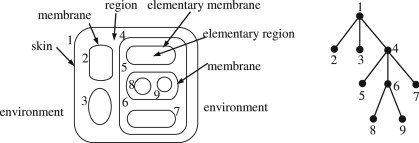
\includegraphics{img/membrane_structure.jpg}
  \caption{The membrane structure of a P system and its associated tree \cite{Zhang20101997AnalyzingRadarSignalsWithMembrane}}
  \label{fig:membrane_structure}
\end{figure}

% Membrane models

Recently, several computational models based on the membrane structure have been created.



% P systems

\subsubsection{P systems} % (fold)
\label{subs:p_systems}

P systems were introduced in 1998 as a system with membrane structure that contains multisets of objects and rewrite rules that are executed in a maximally parallel manner. Since then, a huge amount of variants have been created with various computation powers. We have investigated the power of several such variants. Additionally, we propose a new variant with a vacuum, where the rules can describe what will happen to an object that arrives to an empty membrane.

P systems with existing and newly proposed variants will be discussed in the chapter \ref{cha:p_systems}.

Aside from P systems, other models based on the membrane structure have been created such as the Calculus of Looping Sequences (CLS), which was inspired by P systems.

% subsubsection p_systems (end)


% CLS

\subsubsection{The Calculus of Looping Sequences} % (fold)
\label{subs:calculus_of_looping_sequences}

Barbuti in \cite{Barbuti07CLS} concluded that there is a need for a formalism having a simple notation, having the ability of describing biological systems at different levels of abstractions, having some notions of compositionality and being flexible enough to allow describing new kinds of phenomena as they are discovered, without being specialized to the description of a particular class of systems. The Calculus of Looping Sequences (CLS) was introduced in \cite{Barbuti07CLS}.

The membrane structure in CLS is defined recursively, consisting of terms $T$ and sequences $S$:
$$ T ::= S \mid (S)^L\rfloor T \mid T|T$$
$$ S ::= \eps \mid a \mid S\cdot S $$
, where $a$ is a symbol from the alphabet, $\eps$ represents the empty sequence, $\cdot$ is a sequencing operator, $(S)^L$ is a looping operator, $|$ is a parallel composition operator and $\rfloor$ is a containment operator.

Membranes are represented by a sequence that is looped around.
Several extensions of the CLS have been proposed. In CLS+ the looping operator can be applied to a parallel composition of sequences, which represents a notion of a fluid membrane.
CLS+ can be translated to CLS (see \cite{Barbuti07CLS}).
Milazzo in his PhD thesis \cite{Milazzo07CLS} includes also a simulation of a P system using CLS. The major difficulty is simulating the maximal parallelism of rule application.

% subsubsection calculus_of_looping_sequences (end)

% subsection membrane_systems (end)

% section biologically_inspired_computing_models (end)

% chapter natural_computing (end)

\chapter{P systems} % (fold)
\label{cha:p_systems}

In previous chapter we introduced the notions of membrane and membrane structure.

% Place objects in the regions.

The next step is to place certain objects in the regions delimited by the membranes. The objects are identified by their names, mathematically symbols from a given alphabet.

% Multisets of objects.

Several copies of the same object can appear in a region, so we will work with multisets of objects.

% Evolution rules

In order to obtain a computing device, we will allow the objects to evolve according to evolution rules. Any object, alone or together with another objects, can be transformed in other objects, can pass through a membrane, and can dissolve the membrane in which it is placed.

% Parallelism

All objects evolve at the same time, in parallel manner across all membranes.

% Priorities

The evolution rules are hierarchizes by a priority relation, which is a partial order.

% P system

These aspects all together forms a P system as introduced in \cite{Paun98}. An example of a P system containg rules for computing the Fibonacci sequence can be seen in the figure \ref{fig:p_system_fibonacci}.


In section~\ref{sec:definitions} we will provide formal definition of a P system.

\section{Definitions} % (fold)
\label{sec:definitions}

% Definition taken from my article

{\bf P system} is a tuple $(V, \mu, w_1, w_2,\dots , w_m, R_1, R_2, \dots , R_m)$, where:
\begin{itemize}
  \item $V$ is the alphabet of symbols,
  \item $\mu$ is a membrane structure consisting of $m$ membranes labeled with numbers $1,2,\dots,m$,
  \item $w_1,w_2,\dots w_m$ are multisets of symbols present in the regions $1,2,\dots,m$ of the membrane structure,
  \item $R_1,R_2,\dots R_m$ are finite sets of the rewriting rules associated with the regions $1,2,\dots,m$ of the membrane structure.
\end{itemize}


Each rewriting rule may specify for each symbol on the right side, whether it stays in the current region, moves through the membrane to the parent region or through membrane to one of the child regions. An example of such rule is the following: $abb\rightarrow (a,here)(b,in)(c,out)(c,here)$.

% Configuration

A {\bf configuration} of a P system is represented by its membrane structure and the multisets of objects in the regions.

% Step

A {\bf computation step} of P system is a relation $\Rightarrow$ on the set of configurations such that $C_1 \Rightarrow C_2$ iff:

For every region in $C_1$ (suppose it contains a multiset of objects $w$) the corresponding multiset in $C_2$ is the result of applying a multiset of maximal simultaneously applicable multiset rewriting rules in $R^{msap}_w$ to $w$.

In other words, a maximal multiset of rules is applied in each region.

For example, let's have two regions with multisets $aa$ and $b$. In the first region there is a rule $a\rightarrow b$ and in the second membrane there is a rule $b\rightarrow aa$. The only possible result of a computation step is $bb$, $aa$. The first rule was applied twice and the second rule once. No more object could be consumed by rewriting rules.

% Computation

{\bf Computation} of a P system consists of a sequence of steps. The step $S_i$ is appied to result of previous step $S_{i-1}$. So when $S_i = (C_j,C_{j+1})$, $S_{i-1} = (C_{j-1},C_j)$.

% Result of a computation

There are two possible ways of assigning a result of a computation:

\begin{enumerate}
    \item By considering the multiplicity of objects present in a designated membrane in a halting configuration. In this case we obtain a vector of natural numbers. We can also represent this vector as a multiset of objects or as Parikh image of a language.
    \item By concatenating the symbols which leave the system, in the order they are sent out of the skin membrane (if several symbols are expelled at the same time, then any ordering of them is accepted). In this case we generate a language.
\end{enumerate}

The result of a computation is clearly only one multiset or a string, but for one initial configuration there can be multiple possible computations. It follows from the fact that there exist more than one maximal multiset of rules that can be applied in each step.

\begin{figure}[h]
  \centering
  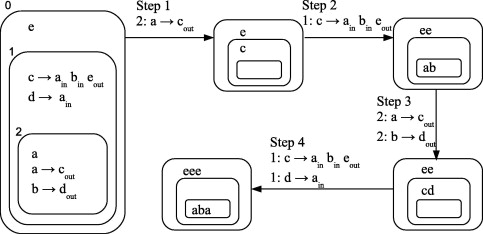
\includegraphics[width=0.8\textwidth]{img/p_system_fibonacci.jpg}
  \caption{P system computing a Fibonacci sequence \cite{Buiu201233PSystemFibonacci}}
  \label{fig:p_system_fibonacci}
\end{figure}

% TODO: quality vs quantity aspects.


% section definitions (end)

\section{P system variants} % (fold)
\label{sec:p_system_variants}
% !TEX root = ../diz.tex
Besozzi in his PhD thesis (see \cite{Besozzi:PhD:2004}) formulates three criteria that a good P system variant should satisfy:

\begin{enumerate}
	\item It should be as much realistic as possible from the biological point of view, in order not to widen the distance between the inspiring cellular reality and the idealized theory.
	\item It should result in computational completeness and efficiency, which would mean to obtain universal (and hence, programmable) computing devices, with a powerful and useful intrinsic parallelism;
	\item It should present mathematical minimality and elegance, to the aim of proposing an alternative framework for the analysis of computational models.
\end{enumerate}

In membrane computing, many models are equal in power with Turing machines. We should say they are Turing complete (or computationally complete), but because the proofs are always constructive, starting the constructions from these proofs from universal Turing machines or from equivalent devices, we obtain universal P systems (able
to simulate any other P system of the given type). That is why we speak about universality results, and not about computational completeness.

\subsection{Accepting vs generating} % (fold)
\label{sub:accepting_vs_generating}

In the Chomsky hierarchy, there are language acceptors (finite automata, Turing machines) and language generators (formal grammars).

% Accepting grammars

Bordhin in \cite{Bordihn99acceptingpure} extends grammars to allow for accepting languages by interchanging the left side with the right side of a rule. The mode will apply rewriting rules to an input word and accept it when it reaches the starting nonterminal. However, the input word consists of terminal symbols, which could not be rewritten when using original definition, hence they consider the pure version of various grammar types where they give up the distinction between terminal and nonterminal symbols.

% Accepting vs generating common results

The regular, context-free, context-sensitive and recursively enumerable languages were shown to have equal power in accepting and generating mode.
Some other grammars (programmed grammars with appearance checking) are shown to be more powerful in accepting mode than in generating mode.
For deterministic Lindenmayer systems, the generating and accepting mode are incomparable.

% Accepting vs generating P system results

It can be interesting to investigate accepting and generating mode also in P system variants. Barbuti in \cite{Barbuti:2010:AcceptingGenerating} shown that in the nondeterministic case, when either promoters or cooperative rules are allowed, acceptor P systems have shown to be universal. The same in known to hold for the corresponding classes of nondeterministic generator P systems. In the deterministic case, acceptor P systems have been shown to be universal only if cooperative rules are allowed. Universality has been shown not to hold for the corresponding classes of generator P systems.

% subsection accepting_vs_generating (end)

\subsection{Active vs passive membranes} % (fold)
\label{sub:active_vs_passive_membranes}

% TODO: need citations
Most of the studied P system variants assumes that the number of membranes can only decrease during a computation, by dissolving membranes as a result of applying evolution rules to the objects present in the system.
A natural possibility is to let the number of membranes also to increase during a computation, for instance, by division, as it is well-known in biology. Actually, the membranes from biochemistry are not at all passive, like those in the models briefly described above.
For example, the passing of a chemical compound through a membrane is often done by a direct interaction with the membrane itself (with the so-called protein channels or protein gates present in the membrane); during this interaction, the chemical compound which passes through membrane can be modified, while the membrane itself can in this way be modified (at least locally).

In \cite{Paun99ActiveMembranes} P\u{a}un considers P systems with active membranes where the central role in the computation is played by the membranes: evolution rules are associated both with objects and membranes, while the communication through membranes is performed with the direct participation of the membranes; moreover, the membranes can not only be dissolved, but they also can multiply by division. An elementary membrane can be divided by means of an interaction with an object from that membrane.

% Polarization

Each membrane is supposed to have an electrical polarization (we will say charge), one of the three possible: positive, negative, or neutral. If in a membrane we have two immediately lower membranes of opposite polarizations, one positive and one negative, then that membrane can also divide in such a way that the two membranes of opposite charge are separated; all membranes of neutral charge and all objects are duplicated and a copy of each of them is introduced in each of the two new membranes.
The skin is never divided.
If at the same time a membrane is divided and there are objects in this membrane which are being rewritten in the same step, then in the new copies of the membrane the result of the evolution is included.

In this way, the number of membranes can grow, even exponentially. As expected, by making use of this increased parallelism we can compute faster.
For example, the SAT problem, which is NP complete, can be solved in linear time, when we consider the steps of computation as the time units.
Moreover, the model is shown to be computationally universal.

% subsection active_vs_passive_membranes (end)

\subsection{Context in rules} % (fold)
\label{sub:context_in_rules}

% Cooperative / Non-cooperative

Rewriting rules in P systems can be cooperative and non-cooperative, like in Chomsky's context-free and context-sensitive grammars. Non-cooperative rules are restricted to use only one object on the left side and cooperative rules do not have this restriction.
P systems with cooperative rules are universal \cite{Paun98}, while P systems with non-cooperative rules only characterize Parikh image of context-free languages ($PsCF$) \cite{Sburlan05dragos}.

% Catalytic P systems

P\u{a}un \cite{Paun98} also defines P systems with catalysts where catalysts are a specified subset of the alphabet. Rewriting rules can contain catalysts, which are not modified by applying the rule. Surprisingly, P systems with catalytic rules are universal, actually two membranes in the P system are sufficient to achieve universality.

In systems where only catalytic rules (purely catalytic systems \cite{Ibarra:03:Catalytic}), three catalysts are enough \cite{Freund2005TwoCatalysts}.

% Two catalysts

Freund in \cite{Freund2005TwoCatalysts} also shows that two catalysts and one membrane are enough and raised an open problem whether one catalyst is sufficient. He conjectured that for computationally universal P systems the results obtained in this paper are optimal not only with respect to the number of membranes (2), but also with respect to the number of catalysts.

% Catalysts are too powerful

From some point of view, catalysts are way too powerful in restricting the parallelism - they directly participate in the rules, hence the number of catalytic rules that can be applied in one step, is bounded by number of catalysts.

A variant with promoters and inhibitors have been proposed (see \cite{Ionescu:jucs_10_5:on_p_systems_with}).

% Promoters

In the case of promoters, the rules are possible only in the presence of certain symbols. An object $p$ is a promoter for a rule $u\rightarrow v$ and we denote this by $u\rightarrow v|_{p}$, if the rule is active only in the presence of object $p$. Note that unlike in the case with catalysts, promoters allow the associated rules to be applied as many times as possible.

% Inhibitors

An object $i$ is inhibitor for a rule $u\rightarrow v$ and we denote this by $u\rightarrow v|_{\neg i}$, if the rule is active only if inhibitor $i$ is not present in the region.
One of our results (see section \ref{sec:inhibitors}) uses inhibitors as a tool to achieve universality for sequential P systems.


% One catalyst with promoters / inhibitors

Ionescu in \cite{Ionescu:jucs_10_5:on_p_systems_with} shows that P systems with non-cooperative catalytic rules with only one catalyst and with promoters / inhibitors are universal.

% Zero catalysts with inhibitors

Non-cooperative rules with no catalysts and with inhibitors were studied in \cite{Sburlan:2006:FurtherResultsPromotersInhibitors}, the equivalence with Lindenmayer systems ($ET0L$ as defined in section \ref{sec:lindenmayer_systems}) was proved.

% Simple cooperative system

Dang \cite{Ibarra04dang} proposes a simple cooperative system ($SCO$) as a P system where the only rules allowed are of the form $a\rightarrow v$ or of the form $aa\rightarrow v$, where $a$ is a symbol and $v$ is a (possibly null) string of symbols not containing $a$. This variant is investigated with various modes of parallelism, so their results will be mentioned in the subsection \ref{sub:parallelism_options}

% subsection context_in_rules (end)

\subsection{Rules with priorities} % (fold)
\label{sub:rules_with_priorities}

In the original definition of a P system \cite{Paun98}, a partial order relation over set of rewriting rules have been specified. The rule can be used only if no rule of a higher priority in the region can be applied at the same time.

Sos\'ik in \cite{Sosik:2002:WithoutPriorities} showed that the priorities may be omitted from the model without loss of computational power.

% subsection rules_with_priorities (end)

\subsection{Energy in P systems} % (fold)
\label{sub:energy_in_p_systems}

Various notions of energy has been proposed for use in P systems. P\u{a}un in \cite{Paun:2001:Energy} considers a P system where each evolution rule ``produces'' or ``consumes'' some quantity of energy, in amounts which are expressed as integer numbers. In each moment and in each membrane the total energy involved in an evolution step should be positive, but if ``Too much'' energy is present in a membrane, then the membrane will be destroyed (dissolved). This variant was investigated in two cases, both were shown to be universal:

\begin{enumerate}
	\item when using only two membranes and unbounded amount of energy,
	\item when using arbitrarily many membranes and a bounded energy associated with rules
\end{enumerate}

Freund in \cite{Freund:2004:SequentialEnergy} introduced a new variant where the rules are assigned directly to membranes (every rule consume objects on one side of the membrane and produce objects on the other side) and every membrane carries an energy value that can be changed during a computation by objects passing through the membrane.

This variant is universal even in sequential mode if we allow priorities on the objects. When omitting the priority relation, only the family of Parikh sets generated by context-free matrix grammars ($PsMAT$ as defined in section \ref{sec:matrix_grammars}) is obtained.

% subsection energy_in_p_systems (end)

\subsection{Symport / antiport rules} % (fold)
\label{sub:symport_antiport_rules}

P\u{a}un in \cite{Paun:2002:SymportAntiport} proposes a new way of communicating between membranes.

Symports allow two chemicals to pass together through a membrane in the same direction using symport rules of type $(ab,in)$ or $(ab,out)$.
Antiports allow two chemicals to pass simultaneously through a membrane in opposite directions using antiport rules of type $(a,in;b,out)$.

Surprisingly, a P system variant, where only the symport / antiport rules are used are computationally complete. Five membranes are enough for this result. If more than two chemicals may collaborate when passing through membranes, two membranes are sufficient for universality. These results are proven in \cite{Paun:2002:SymportAntiport}.

% subsection symport_antiport_rules (end)

\subsection{Parallelism options} % (fold)
\label{sub:parallelism_options}

Original definition of P system (see \cite{Paun98}) uses maximal parallelism when doing a step of computation. There is an obvious biological motivation relying on the assumption that ``if we wait long enough, then all reaction which may take place will take place''. This condition is rather powerful, because it decreases the non-determinism of the system's evolution. For various reasons ranging from looking for more realistic models to just the mathematical challenge, the maximal parallelism was questioned.

% Sequential mode

Dang in \cite{Dang04Sequential} investigates the sequential mode. In each step, from the set of applicable rules across all membrane one is nondeterministically chosen and applied.

\begin{definition}
  \label{def:computation_step_of_a_sequential_P_system}
  A {\bf computation step of a sequential P system} is a relation $\Rightarrow$ on the set of configurations such that $C_1 \Rightarrow C_2$ holds iff there is an applicable rule in a membrane in $C_1$ such that applying that rule can result in $C_2$.
\end{definition}

For purely catalytic systems with 1 membrane, the sequential mode generates only the semilinear sets and thus is strictly weaker than the maximally parallel version.
Sequential version of symport / antiport systems are equivalent to vector addition systems making it strictly weaker than the original maximally parallel version.

Investigation of the sequential mode continues in \cite{Ibarra05Active}. Sequential P system without priorities with cooperative rules with rules for membrane dissolution are not universal by showing they can be simulated by vector addition systems with states (VASS).
This holds even when the membrane creation is allowed for bounded number of created membranes. However, if any number of membranes are allowed to be created, the system becomes universal. This result was shown by simulation of the register machine (see section \ref{sec:register_machines}).

We have further investigated this variant (sequential P system without priorities with cooperative rules) in chapter \ref{cha:on_the_edge_of_universality_of_sequential_p_systems} by allowing rules with inhibitors, which resulted in universality.


% Restricting maximal parallelism

Dang in \cite{Ibarra04dang} proposes several restricted versions of parallelism.
$n${\bf -Max-Parallel} version nondeterministically selects a maximal subset of at most n rules to apply. It is proved that 9{\bf -Max-Parallel} SCO (defined in the subsection \ref{sub:context_in_rules}) is universal.
$\leq n${\bf -Parallel} version is similar, but does not require the condition of a maximal subset of rules. It is shown to be weaker than $n${\bf -Max-Parallel} version.
$n${\bf -Parallel} version requires the size of the subset of rules to apply to be exactly $n$.
All three versions are equal to the sequential mode when $n=1$. For non-universality results, Dang used the proof technique by simulation by vector addition systems. Our future research may be inspired by this technique.

% Minimal parallelism

Ciobanu in \cite{Ciobanu:2007:MinimalParallelism} proposes a minimal parallelism: for each region if at least one rule can be applied, then at least one rule will be applied. The symport / antiport rules variant and variant with active membranes were both shown to be universal.

% Asynchronous

Freund in \cite{Freund:2004:Async} studied the asynchronous mode of P systems, where in each step, arbitrary many rules can be applied. The application of rules is hence done in parallel way, but are not synchronized or somewhat controlled. In many cases the sequential and asynchronous modes were shown to be equivalent.

% subsection parallelism_options (end)


% section p_system_variants (end)

\section{Case studies} % (fold)
\label{sec:case_studies}

\subsection{Vultures in Pyrenees} % (fold)
\label{sub:vultures_in_pyrenees}

Spanish researchers in \cite{Cardona:2009:Vultures} presented a model of an ecosystem related to the Bearded Vulture in Pyrenees in Spain by using P systems. They have constructed a simulator to validate the designed P system, which allows them to analyze the evolution under different initial conditions.

% subsection vultures_in_pyrenees (end)

\subsection{Cellular Signalling Pathways} % (fold)
\label{sub:cellular_signalling_pathways}

Perez in \cite{Perez06EGFR} proposed a model for EGFR Signalling Cascade. More than 60 proteins were included and 160 chemical reactions. Membrane structure consists of 3 regions: the environment, the cell surface and the cytoplasm. 

% subsection cellular_signalling_pathways (end)

\subsection{Solving SAT in linear time} % (fold)
\label{sub:solving_sat_in_linear_time}


Polynomial time solutions to NP-complete problems by means of P systems are achieved by trading time (number of computation steps) for space (number of membranes and objects). This is inspired by the capabililty of cells to produce an exponential number of new membranes in polynomial time.

However, many simulators of P system are inefficient since they cannot handle the parallelism of these devices. Nowadays, we are witnessing the consolidation of the GPUs as a parallel framework to compute general purpose applications such as bitcoin mining. The simulation of P systems with active membranes using GPUs is analysed in \cite{Cecilia10SAT} and an efficient linear solution to the SAT problem is illustrated.

They compared it to the classical simulator and reported up to 94x of speedup for 256 literals in the formula. The major constraint of this parallel simulation is the GPU memory size, which can be overcome with a data partition on a cluster of GPUs. 

% subsection solving_sat_in_linear_time (end)

\subsection{Implementation of P systems in vitro} % (fold)
\label{sub:implementation_of_p_systems_in_vitro}

``In vitro'' are studies in experimental biology that uses components of an organism that have been isolated from their usual biological surroundings in order ot provide a more convenient analysis.

% TODO: citation needed Research Topics Arising from the (Planned) P Systems Implementation Experiment in Technion
There was a planned experiment of computing the Fibonacci sequence using P systems in vitro (see \cite{Gershoni:2008:InVitro}) using test tubes as membranes and DNA molecules as objects, evolving under the control of enzymes.
Number of objects in a multiset was represented by a pre-defined ``mole'' of the substance and synchronization was obtained by ``waiting enough'', such that all reactions that can take place in a test tube actually take place. Hence, the variant where reactions don't cycle is required (Local loop-free P systems).
Communication was done by moving all the relevant objects to the next tube in a mechanical way. The final result was read by spectrometry.

The proposed framework has many difficulties. The notable ones are:

\begin{itemize}
  \item Is there any chance to solve NP-complete problems in this frameworks?
  \item Are LL-free P systems universal?
\end{itemize}


% subsection implementation_of_p_systems_in_vitro (end)

% section case_studies (end)

% chapter p_systems (end)

% part overview_of_the_current_state_of_research(end)

\part{Our research} % (fold)
\label{prt:our_research}

\chapter{Computational power of some P system variants} % (fold)
\label{cha:computational_power_of_some_p_system_variants}

We study several variants of P systems and propose a new variant in accordance with the criteria formulated in \cite{Besozzi:PhD:2004} (see beginning of the section \ref{sec:p_system_variants}).

\section{Sequential P systems without priorities with cooperative rules and inhibitors} % (fold)
\label{sec:sequential_p_systems_without_priorities_with_cooperative_rules_and_inhibitors}

Original definition of P systems with inhibitors (see \cite{Ionescu:jucs_10_5:on_p_systems_with}) allow to use only one inhibitor pre rule, e.g. $u\rightarrow v|_{\neg i}$. Alternative definition (see \cite{Agrigoroaiei:2010:Dissolution}) allow to use whole inhibitor set in the rule like $u\rightarrow v|_{\neg B}$, where $B$ is a set of objects. Such a rule can be applied only if no element of $B$ is present in the region.

For sequential P systems, the following lemma will show the equivalence of these definitions. However, special condition must be fulfilled, the regions with such rules cannot be empty.

% !TEX root = ../diz.tex
\begin{lemma}
\label{lemma:inhibitor_step}
  If there is at least one object present in each region of a P system, rewriting step in P system with inhibitor set can be simulated by multiple consecutive steps of P system with single inhibitor.
\end{lemma}

\begin{dokaz}
  Consider a P system with the alphabet $\Sigma$.
  For each rule $u\rightarrow v|_{\neg B}$, where $B=\{b_1, b_2, \dots ,b_n\}$ we will have rules:
    \begin{align*}
      c\rightarrow&c|GONE_{b}|_{\neg b} \text{~for all~} c\in \Sigma, b\in B \\
      u|GONE_{b_1}|GONE_{b_2}|\dots|GONE_{b_n}\rightarrow&v|GONE_{b_1}|GONE_{b_2}|\dots|GONE_{b_n}
    \end{align*}

\end{dokaz}

Note that symbols $GONE_b$ are created automatically when some object $c$ is present in the region. 

\begin{veta}
  The sequential P system with inhibitors defines the same Parikh image of language as P system with maximal parallelism.
\end{veta}

\begin{dokaz}
  We show that we can simulate maximal parallel step of P system with several steps of sequential P system with inhibitors. The proof is quite technical with some workarounds.

  % Membrane states

  It is important to note that in the maximal parallel step the rewriting occurs in all membranes, so we need to synchronize this process. Every membrane will have a state, represented as an object.

  The $RUN$ state represents that the rewriting still occurs. When there are no more rules to apply, the region has done its maximal parallel step and proceeds to the state $SYNCHRONIZE$. Other states are just technical - we need to implement sending objects between membranes and preparing for the next maximal parallel step by unmarking newly created objects in the current maximal parallel step, which have been marked to prevent double rewriting in one step.

  \begin{itemize}
    \item $RUN$: Rewriting occurs. Objects that are to be sent to the parent membrane are directly sent because the parent membrane is already in $RUN$ or $SYNCHRONIZE$ phase, so the $a^{\prime}$ symbols that are sent don't break anything. But objects that are to be sent down, cannot be sent immediately because child membranes can be in the previous phase waiting to restore symbols from previous step. Current symbols could interfere with them and be rewritten twice in this step. Such objects are only marked as ``to be sent down'': $a^{\downarrow\prime}$

    \item $SYNCHRONIZE$: Rewriting has ended and the membrane is waiting to get signal $SYNCED$ from the parent membrane to continue to the next step.

    \item $SENDDOWN$: Signal $SYNCED$ was caught and now all descendant membranes are in $SYNCHRONIZE$ phase so $a^{\downarrow\prime}$ can be sent down.

    \item $RESTORE$: All $a^{\prime}$ symbols are being restored to $a$, so the next step of rewriting can take place.
  \end{itemize}

  % Rewriting rules

  \begin{itemize}
    \item For every rule $r_i\in R$ such that
      \begin{align*}
        r_i = a_1^{M(a_1)}a_2^{M(a_2)}\dots a_n^{M(a_n)} \rightarrow a_1^{N(a_1)}a_2^{N(a_2)}\dots a_n^{N(a_n)}
      \end{align*}
      we will have the following rules:
      \begin{align*}
        &a_1^{M(a_1)-m_1}\dot{a}_1^{m_1}
        a_2^{M(a_2)-m_2}\dot{a}_2^{m_2}\dots
        a_n^{M(a_n)-m_n}\dot{a}_n^{m_n}|RUN \\
        \rightarrow &a_1^{\prime N(a_1)}a_2^{\prime N(a_2)}\dots a_n^{\prime N(a_n)}|RUN
      \end{align*}
      
      There will be such rule for each $0\leq m_i\leq M(a_i)$. It represents the idea that $\dot{a}$ can be used in rewriting in the same way as $a$. Right side of the rules contains symbols $a^\prime$, that prevents the symbols to be rewritten again.

    \item For every symbol $a\in V$ we will have the following rules:

    $a|RUN \rightarrow \dot{a}|RUN|_{\neg \dot{a}}$

    There will be at most one occurrence of $\dot{a}$.

    \item For every rule $r_i\in R$ there will be a rule that detects if the rule $r_i$ is not applicable. According to left side of the rule $r_i$, symbol $UNUSABLE_i$ will be created when there is not enough objects to fire the rule $r_i$. It means that left side of rule $r_i$ requires more instances of some object than are present in membrane.

    If the left side is of type:
    \begin{itemize}
      \item $a$: It is a context free rule. The rule can't be used if there is no occurrence of $a$ nor $\dot{a}$.

      $RUN \rightarrow UNUSABLE_i|RUN|_{\neg\{UNUSABLE_i, a, \dot{a}\}}$

      \item $ab$: It is a cooperative rule with two distinct objects on the left side. The rule cannot be used if there is one of them missing.

      $RUN \rightarrow UNUSABLE_i|RUN|_{\neg\{UNUSABLE_i, a, \dot{a}\}}$

      $RUN \rightarrow UNUSABLE_i|RUN|_{\neg\{UNUSABLE_i, b, \dot{b}\}}$

      \item $a^2$: It is a cooperative rule with two same objects. The rule can't be used if there is at most one occurrence of the symbol. That happens if there is no occurrence of $a$. There can still be $\dot{a}$, but at most one occurrence.

      $RUN \rightarrow UNUSABLE_i|RUN|_{\neg\{UNUSABLE_i, a\}}$
    \end{itemize}

    \item For every membrane with label $i$ there will be a rule:
    \begin{align*}
      &UNUSABLE_1|UNUSABLE_2|\dots|UNUSABLE_m|RUN \\
      \rightarrow &SYNCHRONIZE|SYNCTOKEN_i\uparrow
    \end{align*}

    If no rule can be used, maximal parallel step in the region is completed hence it goes to the synchronization phase and sends a synchronization token to the parent membrane.

    \item For every membrane there will be a rule:
    \begin{align*}
      &SYNCHRONIZE|SYNCTOKEN_j \\
      \rightarrow &SYNCHRONIZE|SYNCTOKEN_j\uparrow
    \end{align*}

    Membrane resends all synchronization tokens from child membranes to the parent membrane.

    \item In the skin membrane there is a rule which collects all the synchronization tokens from all membranes $1\dots k$ and then sends down signal that synchronization is complete. But before that, there can be some symbols that should be sent down, but they weren't, because the region below could have not started the rewriting phase that time. The result was just marked with $a^{\downarrow\prime}$.
    \begin{align*}
      &SYNCTOKEN_1|\dots|SYNCTOKEN_k|SYNCHRONIZE \\
      \rightarrow &SENDDOWN
    \end{align*}

    \item Every membrane other than skin membrane have to receive the signal to go to the senddown phase:

    $SYNCHRONIZE|SYNCED \rightarrow SENDDOWN$

    \item Every membrane will have rules for every symbol $a\in V$ to send down all unsent objects that should have been sent down:

    $SENDDOWN|a^{\downarrow\prime} \rightarrow SENDDOWN|a^{\prime}\downarrow$

    \item Every membrane will have a rule for detecting when all such objects have been sent and it goes to restore phase:

    $SENDDOWN \rightarrow RESTORE|_{\neg \{a_i^{\downarrow\prime}|1\leq i\leq n\}}$

    \item In the restore phase all symbols $a^{\prime}$ will be rewritten to $a$ in order to be able to be rewritten in the next maximal parallel step:

    $RESTORE|a^{\prime} \rightarrow RESTORE|a$
    
    \item When using lemma~\ref{lemma:inhibitor_step}, there may be some $GONE$ symbols left and now is the time to clear them:

    $RESTORE|GONE_i \rightarrow RESTORE$

    \item When the restore phase ends, it sends down a signal that all membranes have been already synchronized and next phase of rewriting has began in upper membranes:

    $RESTORE \rightarrow RUN|SYNCED\downarrow|_{\neg \{a_i^{\prime}|1\leq i\leq n\}\cup\{GONE_i|1\leq i\leq n\}}$
  \end{itemize}

  \definecolor{run}{rgb}{1,0.5,0}
  \definecolor{restore}{rgb}{0,0.5,0}
  \definecolor{synchronize}{rgb}{0,0,1}
  \definecolor{senddown}{rgb}{1,0,0}
  % Narrow texts in boxes
  \providecommand{\narrow}[1]{\scalebox{.85}[1.0]{#1}}

  \begin{figure}
    \def\svgwidth{\textwidth}
    \input{possible_pairs_of_states_of_parent_and_child_membrane.pdf_tex}
    % 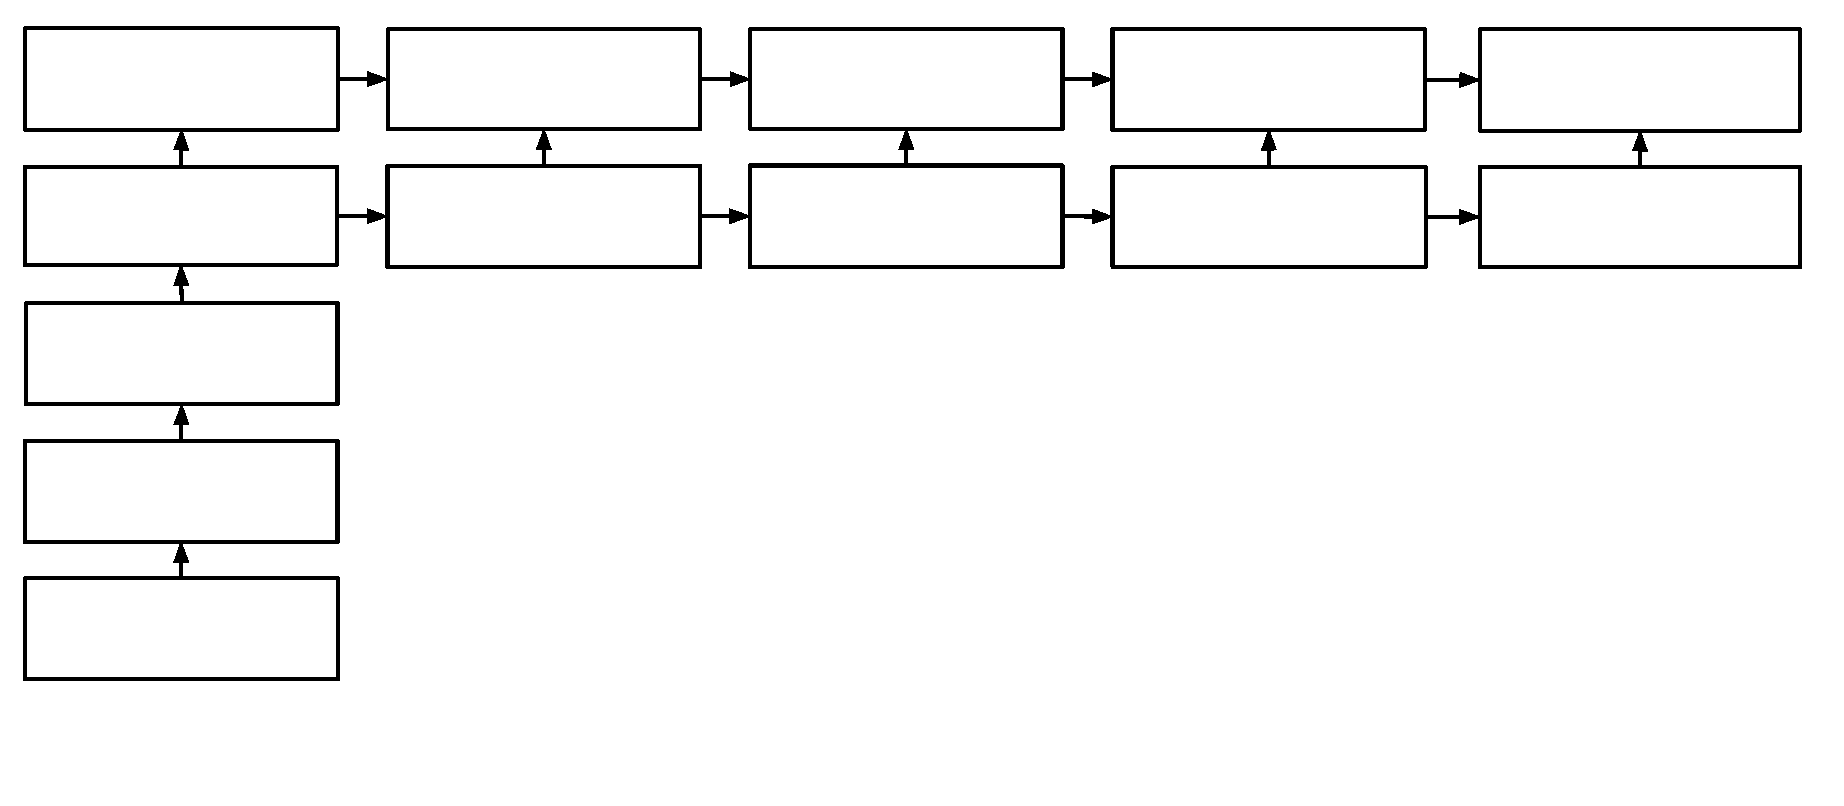
\includegraphics[width=\textwidth]{possible_pairs_of_states_of_parent_and_child_membrane}
    \caption{Possible pairs of states of parent and child membrane}
    \label{fig:possible_pairs_of_states_of_parent_and_child_membrane}
  \end{figure}

  \begin{figure}
    \def\svgwidth{\textwidth}
    \input{snapshot_of_all_membrane_states_while_simulating.pdf_tex}
    % 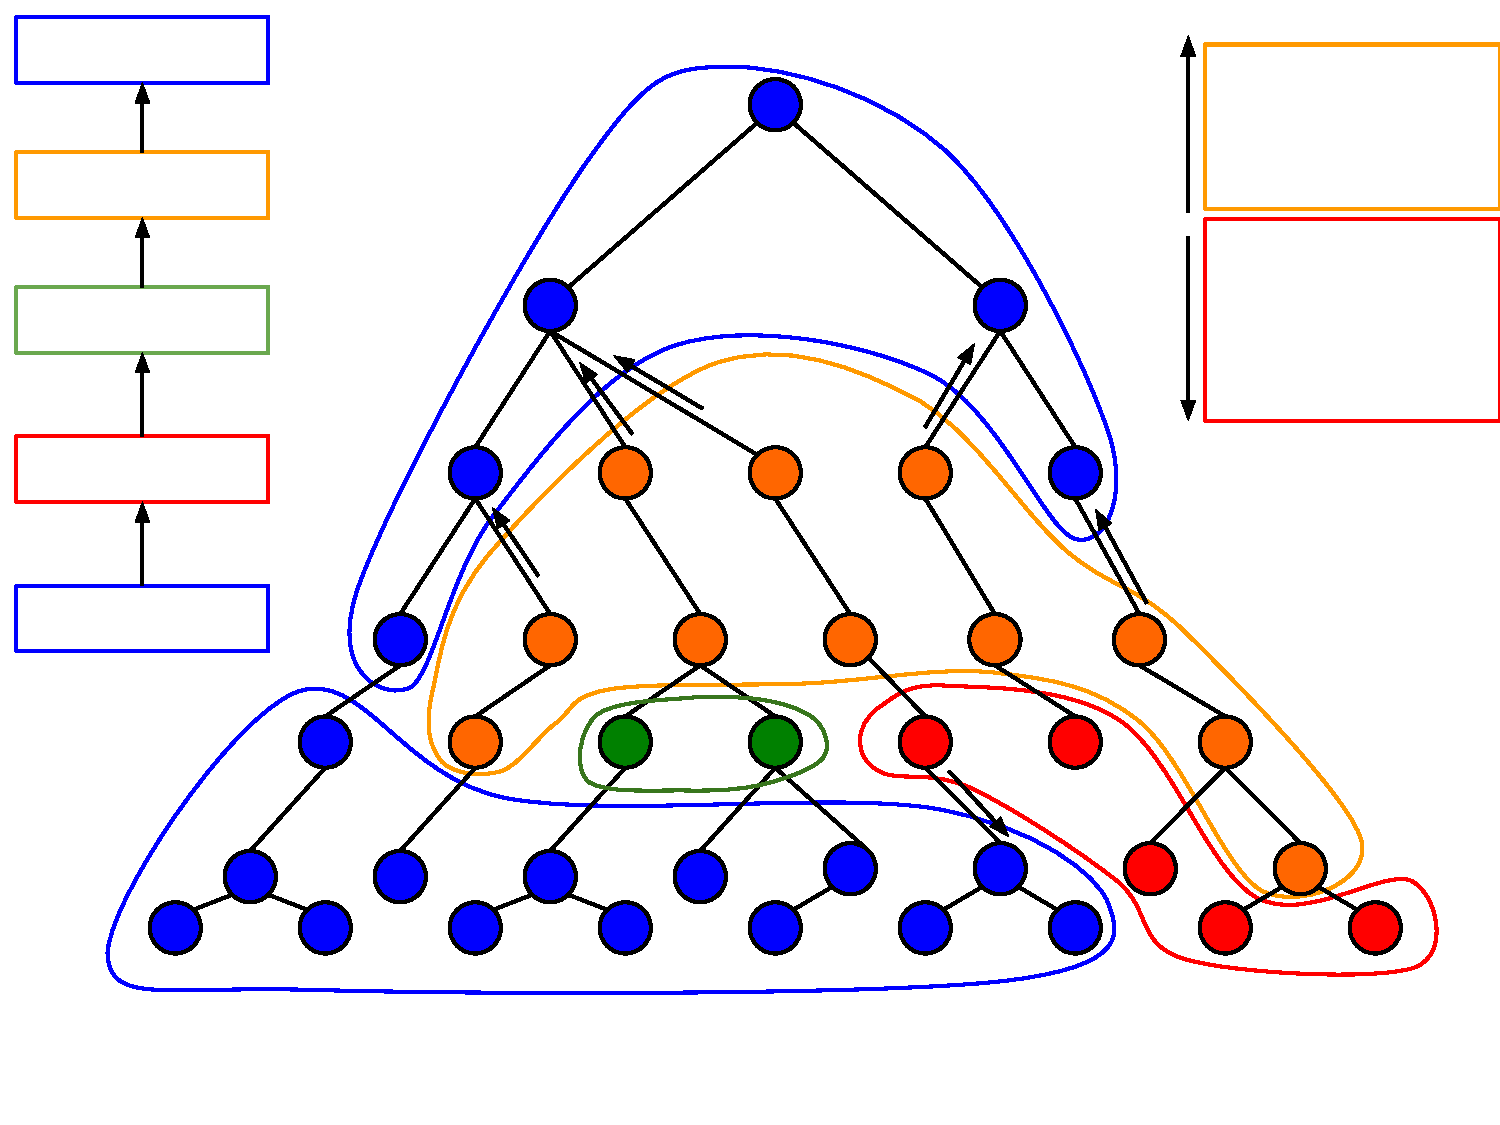
\includegraphics[width=\textwidth]{snapshot_of_all_membrane_states_while_simulating}
    \caption{Snapshot of all membrane states while simulating}
    \label{fig:snapshot_of_all_membrane_states_while_simulating}
  \end{figure}

  The pairs of possible phases of the parent and child membrane are shown in the figure \ref{fig:possible_pairs_of_states_of_parent_and_child_membrane} along with transitions between two consecutive global synchronizations - after the maximal parallel steps $i$ and $i+1$.

  In the figure \ref{fig:snapshot_of_all_membrane_states_while_simulating} the membrane structure is presented as a hierarchical structure. Every membrane is in one of four phases. It can be seen that the sending of the objects is performed in such phases that the receiving membrane is in either $RUN$ or $SYNCHRONIZE$ phase, so the received objects (marked $a^\prime$) does not interfere with rewriting.

  Another interesting idea can be seen in the figure \ref{fig:snapshot_of_all_membrane_states_while_simulating} that when a region is in the $SENDDOWN$ phase and objects are sent through the child membrane, the receiving region is in the $SYNCHRONIZE$ phase waiting for the $SYNCED$ signal, which will be sent to it when $SENDDOWN$ and $RESTORE$ phases finished.

  All membranes are nonempty during the simulation because at least the object representing the current phase is always present. By lemma~\ref{lemma:inhibitor_step} the rules with set of inhibitors can be simulated by single inhibitors.


\end{dokaz}




We have also reached this result in the accepting case by simulation of register machines.

\begin{veta}
  Sequential P systems with inhibitors can simulate register machines and thus equal $PsRE$.
\end{veta}


\begin{dokaz}
\label{proof:reg_by_inh}
  Suppose we have a $n$-register machine $M = (n,P,i,h)$. In our simulation we will have a membrane structure consisting of one membrane and the contents of register $j$ will be represented by the multiplicity of the object $a_j$.

  We will have P system $(V, \mu, w, R)$, where:
  \begin{itemize}
    \item $V$ is an alphabet consisting of symbols that represent registers $a_1,\dots a_n$ and instruction labels in $Lab(M)$,
    \item $\mu$ is a membrane structure consisting of only one membrane,
    \item $w$ is initial contents of the membrane. It contains symbols for the input for the machine $a_i^{n_i}$ where $n_i$ is initial state of register with label $i$ and initial instruction $e \in Lab(M)$.
    \item $R$ is the set of rules in the skin membrane:
    
    For all instructions of type $(e : add(j), f)$ we will have rule:
    \begin{itemize}
      \item $e \rightarrow a_j|f$.
    \end{itemize}
    
    For all instructions of type $(e : sub(j), f, z)$ we will have rules:
    \begin{itemize}
      \item $e|a_j \rightarrow f$ and
      \item $e \rightarrow z|_{\neg a_j}$.
    \end{itemize}

    And finally halting rules:
    \begin{itemize}
      \item $h|a_j \rightarrow h|\#$ for all $a\leq j\leq n$,
      \item $\# \rightarrow \#$,
    \end{itemize}
  \end{itemize}

  When the halting instruction is reached, if there is an object present in the membrane, the hash symbol $\#$ is created and it will cycle forever. If there is no object present, there is no rule to apply and computation will halt. It corresponds to the condition that all registers should be empty when halting.
\end{dokaz}

% section sequential_p_systems_without_priorities_with_cooperative_rules_and_inhibitors (end)

\section{Vacuum} % (fold)
\label{sec:vacuum}

We propose a new variant of P system with vacuum. In the common sense, vacuum represents a state of space with no or a little matter in it. Using vacuum in modelling frameworks can help express certain phenomena more easily. We define a new P system variant, which creates a special vacuum object in a region as soon as the region becomes empty. The vacuum is removed whenever some object interacts with it. After the interaction, there is vacuum no longer. This removal process is realized by allowing the vacuum object to be used only on the left side of rules. If we made the vacuum to be removed automatically when an object enters the region, there would be no difference with the variant without vacuum objects because of no interactions with it.
We are interested in how the variant with the vacuum improves the computation power of a sequential P system in comparison to the variant without using the vacuum.

\begin{veta}
  The sequential P system with Vacuum is universal.
\end{veta}

\begin{dokaz}
  We can simulate the variant of P system where the only cooperative rule is of type $a|a \rightarrow b$. According to \cite{Ibarra04dang} the variant, where the only cooperative rule is when both objects are the same, is universal. If there is no rule $a \rightarrow b$, we can rewrite $a$ to $a^{\prime}$ so we can mark all present symbols. $a^{\prime}$ symbols are kept in special membrane so the Vacuum can be created in main membrane and we can synchronize.
  
  But we won't do this madness again.
  
  Instead, we will try to prove universality by simulating the register machine. We need to detect when the current register is empty. If there was a symbol for every register as in the proof~\ref{proof:reg_by_inh}, the Vacuum would be created only if all registers are empty. But the $sub()$ instruction need to detect when one concrete register is empty.
  
  We will have a membrane for each register. That membrane will be contained in the skin membrane. The number of objects in membrane $i$ will correspond to the value of register $i$.
  
  The alphabet will consist of instruction labels and register counter $a$. The skin membrane will only have an instruction label. It is sent to corresponding membrane where the instruction is executed. Then, the following instruction is sent back to the skin membrane.
  
  We will have following rules in the skin membrane:
  
  \begin{itemize}
  \item $e \rightarrow e\downarrow_j$ for an instruction of type $e : add(j), f$ or $e : sub(j), f, z$ and
  \item $h \rightarrow h\downarrow$ for a halting instruction h.
  \end{itemize}
  
  And in non-skin membranes:
  
  \begin{itemize}
  \item $e \rightarrow a|f\uparrow$ instructions of type $e : add(j), f$,
  \item $e|a \rightarrow f\uparrow$ for instructions of type $e : sub(j), f, z$,
  \item $e|VACUUM \rightarrow z\uparrow$ for instructions of type $e : sub(j), f, z$, and
  \item $h|a \rightarrow h|a$
  \end{itemize}

  When halting, if there is an nonempty register, it will cycle forever with the last rule. However, if all registers are empty, the halting instruction label will stay in all membranes and the computation will halt.
  
\end{dokaz}

% section vacuum (end)

% chapter computational_power_of_some_p_system_variants (end)

% part our_research (end)

\chapter*{Conclusions}
\addcontentsline{toc}{chapter}{Conclusions}
We have studied several variants of sequential P systems in order to obtain universality without using maximal parallelism. A variant with rewriting rules that can use inhibitors was shown to be universal in both generating and accepting case. The generating model is able to simulate maximal parallel P system and the accepting model can simulate a register machine.

In addition, we have defined a new notion of vacuum, which is immediately created in the region that becomes empty. A new P system variant was introduced, which allowed the vacuum to be used on the left side of P system rewriting rules. The accepting case of this variant was shown to be universal by direct implementation of a register machine.

A lot of other variants deserve to be combined with the vacuum, so we suggest to research them more
thoroughly(non-cooperative rules, rules with priorities, decaying objects, deterministic steps, . . . ).
\backmatter

% \begin{thebibliography}{1}
\bibliography{diz}
% \end{thebibliography}

\appendix

\chapter{Štatistiky}
Tu budú štatistiky.

\printindex

\end{document}
